% Unified revision of the constant-contact-rate theory.
% Base: cuizhizhong/optimal-threshold-control@496e454b34f7ce6861238041d5bd14b475e37917
% Original main.tex Git blob: 4ca903f272c8f60ddb308df8f4b550f7364cb971
% Compile from this directory with XeLaTeX + BibTeX.
% Define \TheoryOnly before input to omit the numerical figures and nonautonomous discussion.
\documentclass[11pt,a4paper,UTF8]{ctexart}
\usepackage[a4paper,margin=2.25cm]{geometry}
\usepackage{amsmath,amssymb,amsthm,mathtools,bm}
\usepackage{graphicx}
\usepackage{booktabs,longtable,array,tabularx,multirow}
\usepackage{enumitem,setspace,caption,subcaption,float,placeins,xcolor}
\usepackage{hyperref}
\usepackage[numbers,sort&compress]{natbib}
\usepackage{listings,siunitx,fancyhdr,lastpage}
\graphicspath{{../figures/}}
\setstretch{1.16}
\setlength{\parindent}{2em}
\setlength{\parskip}{0.18em}
\setlist{nosep,leftmargin=2.4em}
\captionsetup{font=small,labelfont=bf}
\hypersetup{colorlinks=true,linkcolor=blue!55!black,citecolor=blue!55!black,
 urlcolor=blue!55!black,pdftitle={跟踪隔离模型中双传播系数的最优控制与唯一性},pdfauthor={Technical report}}
\setlength{\headheight}{14pt}
\pagestyle{fancy}\fancyhf{}
\fancyhead[L]{跟踪隔离模型的最优控制与唯一性}
\fancyhead[R]{\thepage/\pageref{LastPage}}
\renewcommand{\headrulewidth}{0.4pt}
\newtheorem{theorem}{定理}[section]
\newtheorem{proposition}[theorem]{命题}
\newtheorem{lemma}[theorem]{引理}
\newtheorem{corollary}[theorem]{推论}
\newtheorem{assumption}[theorem]{假设}
\theoremstyle{definition}
\newtheorem{definition}[theorem]{定义}
\newtheorem{remark}[theorem]{注}
\newtheorem{example}[theorem]{例}
\newcommand{\R}{\mathbb R}
\newcommand{\Acal}{\mathcal A}
\newcommand{\Dcal}{\mathcal D}
\newcommand{\Gcal}{\mathcal G}
\newcommand{\Uad}{\mathcal U_{\mathrm{ad}}}
\newcommand{\dd}{\,\mathrm d}
\newcommand{\e}{\mathrm e}
\newcommand{\one}{\mathbf 1}
\newcommand{\proj}{\operatorname{Proj}}
\newcommand{\ess}{\operatorname*{ess}}
\newcommand{\argmin}{\operatorname*{arg\,min}}
\lstset{basicstyle=\ttfamily\small,frame=single,breaklines=true,columns=fullflexible,showstringspaces=false}
\title{\bfseries 跟踪隔离模型中双传播系数的最优控制与唯一性\\[2mm]
\large 常接触率的全域 HJB 验证、轨道唯一性与数值分析}
\author{技术分析报告}
\date{2026年9月18日修订稿}
\begin{document}
\maketitle
\ifdefined\TheoryOnly
\begin{center}\small 常接触率理论校样：由同一份 \texttt{main.tex} 编译；省略时变讨论和原工程图形章节。\end{center}
\fi
\begin{abstract}
本文研究由同一跟踪隔离比例驱动、但易感者耗竭和感染者生成系数不同的二维系统。
原始计数变量满足
\[
\dot S=-\beta_1(t)SI,\qquad \dot I=\beta_2(t)SI-\gamma I,
\]
其中 $\beta_1=c(t)[p+(1-p)q]/N$、$\beta_2=pc(t)(1-q)/N$，
$q\in[0,1]$，$0<p<1$。以归一化感染比例 $i\le K$ 为路径状态约束，
最小化线性成本 $J(q)=\int_0^\infty pc(t)q(t)\dd t$。

对常数 $c>0$、$\gamma>0$、$0<K<1$ 及正感染初值，本文先定义所有可测可行控制上的值函数 $V$，
再由自然轨道、容量弧和完全跟踪特征线构造候选成本 $U$。
完全跟踪成本只在其有限可达域内使用。非平凡切换曲线具有严格单调参数化，
并与所有允许的控制方向严格横截。
通过两种等待分支的统一梯度、内部界面的梯度匹配、相对局部 Lipschitz 性，
以及容量水平集上的链式法则，证明沿任意可行轨道的验证不等式。
每条有限成本可行轨道均在有限时间进入无控制安全集，因而全局比较不需要另加未证的无穷远条件。
候选反馈实现下界，故 $U=V$。非平凡最优策略的结构为
$0\to1\to0$ 或 $0\to q_B(s)\to1\to0$，允许初始等待或容量阶段长度为零。
容量等待弧的 Hamiltonian 点态极小集并非单点；本文通过禁止提前离边和分段轨道唯一性，
另证最优控制在全时间轴上几乎处处唯一。

给定时变接触率时，仅保留非自治 HJB、条件性的唯一性判据和正则化的点态投影公式，
不把点态严格凸性或离散求解收敛解释为连续问题的全局唯一性证明。
原工程数值图表用于说明及计算复核，与解析证明的证据范围分别陈述。
\end{abstract}
\noindent\textbf{关键词：} 跟踪隔离；最优控制；状态约束；HJB 验证；切换曲线；几乎处处唯一性
\tableofcontents\newpage

\section{问题来源与建模目标}
\label{sec:model}
Miclo、Spiro 与 Weibull 研究标准 SIR 约化系统中同一个传播函数同时控制易感者减少和感染者增加的情形，
以传播函数低于自然水平的幅度作为线性抑制成本\citep{MicloSpiroWeibull2022}。
本文借鉴其期刊版附录 A.1--A.2 的候选函数验证框架，以及
\citet[\S5.1.4]{Liberzon2012} 的充分性论证，而不直接移用原模型的反馈或唯一性结论。
本模型中两个传播系数由同一控制耦合，且随控制变化的方向相反。

计数变量的二维系统为
\begin{equation}
\begin{cases}
\dot S(t)=-\beta_1(t)S(t)I(t),\\
\dot I(t)=\beta_2(t)S(t)I(t)-\gamma I(t),
\end{cases}
\label{eq:count-model}
\end{equation}
其中
\begin{equation}
\beta_1(t)=\frac{c(t)[p+(1-p)q(t)]}{N},\qquad
\beta_2(t)=\frac{pc(t)(1-q(t))}{N}.
\label{eq:beta12}
\end{equation}
这里 $p\in(0,1)$ 是单次接触传播概率，$c(t)>0$ 是给定接触率，$q(t)\in[0,1]$ 是跟踪隔离比例。
$q$ 增大时，新感染生成系数下降，但未隔离易感者移出的系数上升。
令 $s=S/N$、$i=I/N$，得到
\begin{equation}
\begin{cases}
\dot s=-c(t)[p+(1-p)q]si,\\
\dot i=[pc(t)(1-q)s-\gamma]i.
\end{cases}
\label{eq:normalized-model}
\end{equation}
固定恢复率 $\gamma>0$，要求
\begin{equation}
0<i(t)\le K<1,
\label{eq:capacity}
\end{equation}
并最小化
\begin{equation}
J(q)=\int_0^\infty pc(t)q(t)\dd t.
\label{eq:linear-cost}
\end{equation}
成本是一个取值于 $[0,+\infty]$ 的非负积分；乘以正常数不改变最优控制。

\begin{definition}[控制类与唯一性的含义]
\label{def:admissible}
给定正初值 $x_0=(s_0,i_0)$，其中 $s_0+i_0\le1$、$i_0\le K$。
允许的控制为所有 Lebesgue 可测的 $q:[0,\infty)\to[0,1]$。
其 Carath\'eodory 解全程满足 \eqref{eq:capacity} 时，称控制可行，记作 $q\in\Uad(x_0)$。
控制按几乎处处相等识别。所谓唯一，是指从同一初值出发的任意两个最优控制几乎处处相等，
而不是规定孤立切换瞬间的控制代表元。
\end{definition}

\begin{remark}[结果的适用范围]
本稿常接触率主定理仅讨论 \eqref{eq:normalized-model}、\eqref{eq:linear-cost} 及完整控制区间 $[0,1]$。
不包含感染成本、隔离者回流、折现、控制变化率惩罚或 $q_{\max}<1$。
时变接触率和正则化另行讨论，不能通过改写符号直接继承常接触率主定理。
\end{remark}

\section{解的适定性、正性与基本耗散}
\label{sec:wellposed}
\begin{theorem}[全局解与正性]
\label{thm:wellposed}
设 $c$ 可测且局部本质有界，$c(t)>0$ 几乎处处，$q$ 可测、取值于 $[0,1]$，$s_0,i_0>0$。
则 \eqref{eq:normalized-model} 存在唯一全局 Carath\'eodory 解，满足
\begin{align}
s(t)&=s_0\exp\left[-\int_0^t c(\tau)[p+(1-p)q(\tau)]i(\tau)\dd\tau\right]>0,
\label{eq:s-positive}\\
i(t)&=i_0\exp\left[\int_0^t[pc(\tau)(1-q(\tau))s(\tau)-\gamma]\dd\tau\right]>0,
\label{eq:i-positive}\\
\frac{\dd}{\dd t}(s+i)&=-c(t)q(t)si-\gamma i\le-\gamma i\quad\text{几乎处处}.
\label{eq:sum-decay}
\end{align}
特别地，$s+i\le s_0+i_0$，且
\begin{equation}
\int_0^\infty i(t)\dd t\le\frac{s_0+i_0}{\gamma}.
\label{eq:i-integrable}
\end{equation}
若 $c$ 全局有界，则 $i(t)\to0$。
\end{theorem}
\begin{proof}
右端关于状态局部 Lipschitz，时间相关的局部界可积，故局部解存在唯一。
对正性公式积分，并将两方程相加，即得以上关系。
非负状态被限制在 $s+i\le s_0+i_0$ 的有界三角形内，不发生有限时间爆破，解可延拓至所有有限时间。
若 $c$ 有界，则 $\dot i$ 有界，故 $i$ 一致连续；非负一致连续且可积的函数趋于零。
最后一条可直接反证：若存在无穷多个 $i(t_n)\ge\epsilon>0$，一致连续性给出互不相交、长度一致正的区间，
使 $\int i=\infty$，矛盾。
\end{proof}

\section{常接触率问题、自然轨道与安全目标集}
\label{sec:constant-problem}
从本节至第\ref{sec:constant-uniqueness}节固定
\begin{equation}
c>0,\quad\gamma>0,\quad0<p<1,\quad0<K<1,
\qquad h=\frac{\gamma}{pc},\quad\ell=\frac{\gamma}{c}=ph,\quad r=(1-p)h,
\label{eq:constants}
\end{equation}
所以 $h=r+\ell$、$0<r<h$。
物理可行状态域为
\begin{equation}
\Dcal=\{(s,i):s>0,\ 0<i\le K,\ s+i\le1\},\qquad
V(x)=\inf_{q\in\Uad(x)}J_x(q).
\label{eq:value-definition}
\end{equation}
此处的下确界没有预先限制控制的切换次数或取值结构。
为方便几何参数化，先在辅助正条带
$\Omega=\{s>0,\ 0<i\le K\}$ 中定义各曲线和候选函数，再限制到 $\Dcal$。
超出 $s+i\le1$ 的辅助曲线不是实际允许的状态；实际候选轨道保持 $s+i\le1$，
这是定理\ref{thm:wellposed}的结论，而非额外假设。

\subsection{自然传播不变量与峰值}
$q=0$ 时
\begin{equation}
\dot s=-pcsi,\qquad \dot i=pc(s-h)i.
\label{eq:q0-system}
\end{equation}
定义
\begin{equation}
\Phi(s,i)=i+s-h\ln s.
\label{eq:Phi}
\end{equation}
直接求导得 $\dot\Phi=0$。经过 $(s_0,i_0)$ 的自然轨道为
\begin{equation}
i_{\rm nat}(s)=i_0+s_0-s+h\ln\frac{s}{s_0}.
\label{eq:natural-orbit}
\end{equation}
若 $s_0>h$，则自然感染峰值在 $s=h$ 处取得：
\begin{equation}
i_{\rm pk}=i_0+s_0-h+h\ln\frac h{s_0}.
\label{eq:natural-peak}
\end{equation}
若 $s_0\le h$，感染从初始时刻起不增。

\subsection{安全集与目标边界}
记
\begin{equation}
\Phi_A=K+h-h\ln h,\qquad
 a(s)=\Phi_A-s+h\ln s\quad(s\ge h).
\label{eq:safe-boundary}
\end{equation}
辅助条带中的安全集及物理安全集分别为
\begin{equation}
\widehat{\Acal}=\Omega\cap\bigl(\{s\le h\}\cup\{s>h,\ \Phi\le\Phi_A\}\bigr),
\qquad \Acal=\widehat{\Acal}\cap\Dcal.
\label{eq:safe-set}
\end{equation}
以下在辅助几何中使用 $\widehat{\Acal}$，实际控制问题的目标集始终是 $\Acal$。

\begin{proposition}[最大无控制安全集]
\label{prop:safe-exact}
对 $x\in\Dcal$，$x\in\Acal$ 当且仅当从 $x$ 出发永久取 $q=0$ 时始终有 $i\le K$。
因此 $V=0$ 于 $\Acal$，唯一的零成本控制为 $q=0$ 几乎处处。
\end{proposition}
\begin{proof}
由 \eqref{eq:natural-peak} 以及 $s\le h$ 时感染不增，得到安全性的充要条件。
$q=0$ 的成本为零，非负成本不可能更低；$pc>0$ 保证零成本等价于 $q=0$ 几乎处处。
\end{proof}

\section{两类控制弧与显式成本}
\label{sec:arcs}
\subsection{一般控制下的不变量导数}
直接代入状态方程得
\begin{equation}
\boxed{\dot\Phi=-cqi(s-r).}
\label{eq:Phi-derivative}
\end{equation}
定义 $\Psi(s,i)=i-\ell\ln s$，同样得到
\begin{equation}
\dot\Psi=pc(1-q)i(s-r).
\label{eq:Psi-derivative}
\end{equation}
这两个单调性只在 $s>r$ 的区域按所示方向成立；本稿使用它们时均处于 $s>h>r$。

\begin{lemma}[安全集对控制的前向不变性]
\label{lem:safe-invariant}
从 $\widehat{\Acal}$ 出发的任意 $[0,1]$ 值控制均保持在 $\widehat{\Acal}$；在物理域中相应保持在 $\Acal$。
\end{lemma}
\begin{proof}
只要 $s>h$，\eqref{eq:Phi-derivative} 保证 $\Phi$ 不增，故 $i\le a(s)\le K$。
一旦 $s\le h$，因 $s$ 不增，且 $\dot i\le pc(s-h)i\le0$，安全性永久保持。
物理总量约束由 \eqref{eq:sum-decay} 保持。
\end{proof}

\subsection{完全跟踪弧}
$q=1$ 时
\begin{equation}
\dot s=-csi,\qquad \dot i=-\gamma i,
\label{eq:q1-system}
\end{equation}
因此
\begin{equation}
\boxed{\Psi(s,i)=i-\ell\ln s\quad\text{沿 }q=1\text{ 保持不变}.}
\label{eq:Psi}
\end{equation}
由 $(s_a,i_a)$ 到 $(s_b,i_b)$ 的弧满足
\begin{align}
i_b-\ell\ln s_b&=i_a-\ell\ln s_a,
\label{eq:q1-characteristic}\\
i(t)&=i_a\e^{-\gamma(t-t_a)},
\label{eq:q1-i}\\
s(t)&=s_a\exp[-(i_a-i(t))/\ell].
\label{eq:q1-s}
\end{align}
若终点感染 $i_b>0$，所需时间与成本有限，且
\begin{equation}
\int_{t_a}^{t_b}pc\dd t=\frac1h\ln\frac{i_a}{i_b}.
\label{eq:q1-cost}
\end{equation}

\subsection{容量弧}
\label{sec:boundary-arc}
在 $i=K$ 上，不能向 $i>K$ 运动，故边界允许的瞬时方向对应
\begin{equation}
Q_K(s)=\left[\max\{0,1-h/s\},\ 1\right].
\label{eq:boundary-feasible}
\end{equation}
当 $s>h$ 时，唯一切向控制是
\begin{equation}
\boxed{q_B(s)=1-h/s.}
\label{eq:qB}
\end{equation}
$q>q_B$ 也可行，但会进入容量下方；不能在问题定义中直接排除它。
沿 $q_B$ 有
\begin{align}
\dot i&=0,\label{eq:boundary-i}\\
\dot s&=-cK(s-r),\label{eq:boundary-s}\\
s(t)&=r+(s_a-r)\e^{-cK(t-t_a)}.\label{eq:boundary-s-explicit}
\end{align}
对 $s_{\rm hi}\ge s_{\rm lo}\ge h$，
\begin{equation}
T_B(s_{\rm hi},s_{\rm lo})=\frac1{cK}\ln\frac{s_{\rm hi}-r}{s_{\rm lo}-r},
\label{eq:boundary-duration}
\end{equation}
\begin{align}
C_B(s_{\rm hi},s_{\rm lo})
&=\frac pK\int_{s_{\rm lo}}^{s_{\rm hi}}\frac{s-h}{s(s-r)}\dd s\notag\\
&=\frac{p}{K(1-p)}\left[\ln\frac{s_{\rm hi}}{s_{\rm lo}}
-p\ln\frac{s_{\rm hi}-r}{s_{\rm lo}-r}\right].
\label{eq:boundary-cost}
\end{align}
这些式子是指定容量策略的成本计算，尚不是其最优性结论。

\section{有限成本可行性与首次到达问题}
\label{sec:exit-time}
\begin{lemma}[有限成本比较策略]
\label{lem:finite-feasible}
对每个 $x_0\in\Dcal$，存在有限成本可行控制，因而 $V(x_0)<\infty$。
\end{lemma}
\begin{proof}
安全初值采用 $q=0$。否则 $s_0>h$、$i_{\rm pk}>K$。
若 $i_0<K$，自然轨道在到达 $s=h$ 之前首次到达容量，触点记为 $(s_1,K)$，其中 $h<s_1<s_0$。
其时间有限：在到达 $s=h$ 或容量之前 $i\ge i_0$，所以 $\dot s\le-pci_0s$。
若始终不到达二者，后一估计会使 $s<h$，矛盾；不安全性又排除了先到 $h$ 而未到容量。
若 $i_0=K$，取 $s_1=s_0$。
随后沿容量弧运行至 $(h,K)$，再永久采用 $q=0$。
容量弧时间与成本由 \eqref{eq:boundary-duration}--\eqref{eq:boundary-cost} 有限。
全程可行，且总量约束保持。自然触点满足
\begin{equation}
K=i_0+s_0-s_1+h\ln\frac{s_1}{s_0}.
\label{eq:s1}
\end{equation}
\end{proof}

\begin{lemma}[所有有限成本轨道均在有限时间进入安全集]
\label{lem:finite-entry}
若 $q\in\Uad(x_0)$ 且 $J(q)<\infty$，则
$\tau_{\Acal}(x_0,q):=\inf\{t\ge0:x_q(t)\in\Acal\}<\infty$。
更强地，从 $s_0>h$ 出发时，存在有限 $T_h$ 使 $s(T_h)\le h$。
\end{lemma}
\begin{proof}
常接触率下 $J(q)<\infty$ 等价于 $\int_0^\infty q\dd t<\infty$。
假设 $s_0>h$，但对所有有限 $t$ 都有 $s(t)>h$。
由正性及状态方程，
\begin{align*}
\ln\frac{i(t)}{i_0}
&=pc\int_0^t(s(\tau)-h)\dd\tau-pc\int_0^t s(\tau)q(\tau)\dd\tau\\
&\ge-pcs_0\int_0^\infty q(\tau)\dd\tau.
\end{align*}
于是 $i(t)\ge i_0\exp[-pcs_0\int_0^\infty q\dd t]>0$，与 \eqref{eq:i-integrable} 矛盾。
故有限 $T_h$ 存在；可行性给出 $i(T_h)\le K$，所以 $x(T_h)\in\Acal$。
$s_0\le h$ 时初值已经安全。$\Acal$ 在正状态域相对闭，轨道连续，故有限首次到达时刻确实到达目标集。
\end{proof}

\begin{proposition}[无穷时域与首次到达问题等价]
\label{prop:exit-equivalence}
令 $\mathcal U_{\Acal}(x)$ 为有限时间内保持可行并到达 $\Acal$ 的可测控制类，以首次到达为截断时刻。
则
\begin{equation}
V(x)=\inf_{q\in\mathcal U_{\Acal}(x)}
\int_0^{\tau_{\Acal}(x,q)}pcq(t)\dd t.
\label{eq:exit-value}
\end{equation}
\end{proposition}
\begin{proof}
任意有限到达控制可接上 $q=0$，形成相同成本的无穷时域可行控制。
反之，任意有限成本无穷时域控制由引理\ref{lem:finite-entry}可在首次到达时截断，成本不增加。
无穷成本控制不会降低已知有限的下确界。两个方向给出等式。
\end{proof}
\begin{remark}[终点与停止付费]
对不安全初值，首次到达必位于 $i=a(s)$ 的正感染部分，且 $s\ge h$。
这是目标集约束，不是固定终点或固定终止时间；无需 $i=0$，也无需 $s=h$。
首次到达后，$q=0$ 是零成本可行延拓。若允许在安全集内继续等待再宣布终止，记录的终止时间可不唯一，
这不属于控制在几乎处处意义下的非唯一性。
\end{remark}

\section{HJB 方程与验证所需的边界条件}
\label{sec:HJB}
记
\begin{align}
f_0(s,i)&=(-pcsi,\ pc(s-h)i),\label{eq:f0}\\
f_1(s,i)&=(-csi,\ -\gamma i),\label{eq:f1}\\
f_q&=(1-q)f_0+qf_1.\label{eq:control-affine}
\end{align}
对可微函数 $Z$ 定义含运行成本的 Hamiltonian
\begin{equation}
H_Z(x,q)=\nabla Z(x)\cdot f_q(x)+pcq
=H_{0,Z}(x)+q\Sigma_Z(x),
\label{eq:H-affine}
\end{equation}
其中
\begin{align}
H_{0,Z}&=-pcsiZ_s+pc(s-h)iZ_i,\label{eq:H0}\\
\Sigma_Z&=pc-csi[(1-p)Z_s+pZ_i].\label{eq:switching-function}
\end{align}
在不安全区域内部，动态规划在可微点导出
\begin{equation}
\min_{0\le q\le1}\{\nabla V\cdot f_q+pcq\}=0.
\label{eq:HJB}
\end{equation}
目标集上为 $V=0$。在 $i=K,s>h$ 上，若具有适当内侧导数，边界经典形式是
\begin{equation}
\min_{q\in Q_K(s)}\{\nabla V(s,K)\cdot f_q(s,K)+pcq\}=0.
\label{eq:boundary-HJB}
\end{equation}
这里不预设 $V(s,K)=0$、$V_i(s,K)=0$ 或 $q=q_B$。
严格的状态约束 HJB 理论需区分边界方向与目标数据；
本稿不预设 $V$ 的可微性，也不依赖一个未经检验的黏性解比较定理，
而是直接对构造出的 $U$ 证明沿任意可行轨道的积分不等式。
这一充分性逻辑与 \citet[附录 A.1]{MicloSpiroWeibull2022} 及
\citet[\S5.1.4]{Liberzon2012} 一致，但下文的非光滑处理和具体分区由本模型单独证明。

\begin{lemma}[仿射 Hamiltonian 的点态极小]
\label{lem:bangbang}
内部点若 $\Sigma_Z>0$，唯一极小元为 $q=0$；若 $\Sigma_Z<0$，唯一极小元为 $q=1$。
若 $\Sigma_Z=0$，整个 $[0,1]$ 都是点态极小集。
边界上将 $[0,1]$ 换为 $Q_K(s)$。
\end{lemma}
\begin{proof}
由 \eqref{eq:H-affine} 关于 $q$ 的仿射性直接得到。
这只是固定状态与梯度下的结论，不能单独排除奇异弧或证明轨道唯一。
\end{proof}

\section{完全跟踪成本的有限可达域及导数}
\label{sec:q1-value}
令 $s_K>h$ 为 $a(s_K)=0$ 的唯一根。
存在唯一性由 $a(h)=K>0$、$a'(s)=(h-s)/s<0$ 和 $a(s)\to-\infty$ 得到。

\begin{proposition}[正感染端点存在的充要条件]
\label{prop:reachable}
对 $x=(s,i)\in\Omega\setminus\widehat{\Acal}$，立即取 $q=1$ 能在有限时间进入安全集，当且仅当
\begin{equation}
x\in\mathcal E:=\{x\in\Omega\setminus\widehat{\Acal}:s\e^{-i/\ell}<s_K\}
=\{x\in\Omega\setminus\widehat{\Acal}:i>\ell\ln(s/s_K)\}.
\label{eq:reachable}
\end{equation}
此时唯一首次端点 $(\bar s,\bar i)$ 满足 $h<\bar s<s$、$0<\bar i=a(\bar s)<i$，以及
\begin{equation}
\begin{cases}
\bar i=a(\bar s),\\ i-\ell\ln s=\bar i-\ell\ln\bar s,
\end{cases}
\label{eq:endpoint-system}
\end{equation}
等价于
\begin{equation}
\Phi_A-\bar s+r\ln\bar s=i-\ell\ln s.
\label{eq:endpoint-root}
\end{equation}
\end{proposition}
\begin{proof}
完全跟踪轨道的极限为 $(s_\infty,0)$，其中 $s_\infty=s\e^{-i/\ell}$。
若 $s_\infty\ge s_K$，全程 $s(t)>s_\infty>h$，且
$\Phi(t)>s_\infty-h\ln s_\infty\ge\Phi_A$，故不到达安全集。
若 $h\le s_\infty<s_K$，则 $\Phi(t)$ 严格下降至小于 $\Phi_A$ 的极限，有限时间内穿过 $\Phi_A$。
若 $s_\infty<h$，则有限时间到达 $s=h$，该时 $i<K$，故在此之前已穿过安全边界。
在等号 $s_\infty=h$ 的情形，前一种论证同样适用。
端点必满足 \eqref{eq:endpoint-system}；函数 $G(z):=a(z)-\ell\ln z$ 在 $z>h$ 上有
$G'(z)=(r-z)/z<0$，从而端点唯一。
又 $i<K$ 在任何正长度完全跟踪弧的末端严格成立，故首次安全端点不可能是 $(h,K)$，于是 $\bar s>h$。
\end{proof}

\begin{definition}[指定完全跟踪策略的成本]
\label{def:W}
在 $\mathcal E$ 上定义
\begin{equation}
W(s,i)=\frac1h\ln\frac{i}{\bar i(s,i)}.
\label{eq:W}
\end{equation}
在不安全但不属于 $\mathcal E$ 的点，将\emph{立即完全跟踪直至安全集这一指定方案}的成本记为 $+\infty$。
这不表示原问题的 $V=+\infty$；引理\ref{lem:finite-feasible}已经给出有限成本比较策略。
\end{definition}
端点映射在 $\mathcal E$ 内光滑，隐式求导得到
\begin{equation}
\bar s_s=\frac{\ell\bar s}{s(\bar s-r)},\qquad
\bar s_i=-\frac{\bar s}{\bar s-r},
\label{eq:endpoint-derivatives}
\end{equation}
从而
\begin{align}
W_s&=\frac{\ell(\bar s-h)}{hs(\bar s-r)\bar i}
=\frac p s\Theta(\bar s,\bar i),\label{eq:Ws}\\
W_i&=\frac1h\left[\frac1i-\frac{\bar s-h}{(\bar s-r)\bar i}\right]
=\frac1h\left[\frac1i-\Theta(\bar s,\bar i)\right],\label{eq:Wi}
\end{align}
其中
\begin{equation}
\Theta(s,i)=\frac{s-h}{i(s-r)},\qquad s>h,
\label{eq:Theta}
\end{equation}
并记
\begin{equation}
D(s,i)=\Theta(\bar s,\bar i)-\Theta(s,i)\quad(x\in\mathcal E).
\label{eq:D-residual}
\end{equation}
这里的标量 $D$ 不要与状态域 $\Dcal$ 混淆。

\begin{proposition}[完全跟踪成本的 Hamiltonian 恒等式]
\label{prop:W-HJB}
在 $\mathcal E$ 上，
\begin{align}
H_W(x,1)&=\nabla W\cdot f_1+pc=0,\label{eq:H1-zero}\\
H_W(x,0)&=\frac{pc}{h}i(s-r)[\Theta(s,i)-\Theta(\bar s,\bar i)]
=-\frac{pc}{h}i(s-r)D(s,i).\label{eq:H0-theta}
\end{align}
特别地，$D<0$ 时所有 $q$ 均有 $H_W(x,q)\ge0$，等号仅在 $q=1$ 成立。
\end{proposition}
\begin{proof}
将 \eqref{eq:Ws}--\eqref{eq:Wi} 代入 $f_1$，用 $\gamma=pch$、$\ell=ph$ 即得第一式。
代入 $f_0=pci(-s,s-h)$，并用 $ph+s-h=s-r$，得到第二式。
因 $H_W(x,q)=(1-q)H_W(x,0)$，最后一条随即成立。
\end{proof}

\section{切换曲线的存在、单调性及严格横穿}
\label{sec:switching-curve}
固定安全端点 $z\in(h,s_K)$，沿反向完全跟踪特征线写成
\begin{equation}
I_z(s)=a(z)+\ell\ln(s/z),\qquad s\ge z.
\label{eq:q1-backward}
\end{equation}
定义
\begin{equation}
g(s)=\frac{(s-h)(s-r)}s=s-h-r+\frac{hr}{s}.
\label{eq:g}
\end{equation}

\begin{lemma}[单峰性及非平凡根的参数域]
\label{lem:unimodal}
沿 \eqref{eq:q1-backward} 有
\begin{align}
\frac{\dd}{\dd s}\ln\Theta(s,I_z(s))
&=\ell\left[\frac1{(s-h)(s-r)}-\frac1{sI_z(s)}\right],
\label{eq:theta-log-derivative}\\
\frac{\dd}{\dd s}(g(s)-I_z(s))
&=\frac{(s-h)(s+r)}{s^2}>0.
\label{eq:g-minus-i}
\end{align}
存在唯一 $e\in(h,s_K)$ 使 $a(e)=g(e)$。
方程
\begin{equation}
\Theta(s,I_z(s))=\Theta(z,a(z))
\label{eq:switch-condition}
\end{equation}
具有非平凡根 $s>z$ 当且仅当 $h<z<e$；此时该根唯一，记为 $\sigma(z)$，并有
$I_z(\sigma(z))<g(\sigma(z))$。
\end{lemma}
\begin{proof}
两条导数由直接求导得到，第一条的符号与 $I_z-g$ 相同。
$a$ 在 $(h,s_K)$ 严格下降，而 $g$ 严格上升，且
$a(h)-g(h)=K>0$、$a(s_K)-g(s_K)<0$，故 $e$ 存在唯一。
若 $z<e$，$I_z(z)>g(z)$，而 $g-I_z$ 严格上升并趋于 $+\infty$，
所以 $\Theta(s,I_z(s))$ 先严格上升后严格下降，其极限为零。
它恰好一次返回正的初始值，返回点严格在峰点右侧。
若 $z\ge e$，则在 $s>z$ 上 $I_z<g$，$\Theta$ 严格下降，不可能返回初始值。
\end{proof}

\begin{proposition}[非平凡切换曲线的全分支]
\label{prop:Gamma-geometry}
令 $j(z)=I_z(\sigma(z))$，$h<z<e$。
则 $\sigma,j$ 在该开区间上光滑，且
\begin{equation}
\sigma'(z)<0,\qquad j'(z)<0.
\label{eq:sigma-monotone}
\end{equation}
完整辅助切换曲线
\begin{equation}
\Gamma_\infty=\{(\sigma(z),j(z)):h<z<e\}
=\{(s,I_\Gamma(s)):e<s<\infty\}
\label{eq:switch-param}
\end{equation}
是简单光滑曲线，满足
\begin{equation}
I_\Gamma'(s)>\ell/s>0,
\qquad
\lim_{s\downarrow e}I_\Gamma(s)=a(e),\quad
\lim_{s\to\infty}I_\Gamma(s)=\infty.
\label{eq:Gamma-slope}
\end{equation}
在 $z\uparrow e$ 时，$\sigma(z)\to e$、$j(z)\to a(e)$；不在此合并端点直接使用隐函数定理。
\end{proposition}
\begin{proof}
取特征线标号 $\psi=G(z)=a(z)-\ell\ln z$，有 $\psi'(z)=(r-z)/z<0$。
设 $L(s,\psi)=\ln[(s-h)/(s-r)]-\ln(\psi+\ell\ln s)$。
根方程为 $F(s,\psi)=L(s,\psi)-L(z(\psi),\psi)=0$。
由引理\ref{lem:unimodal}，非平凡根处 $F_s<0$，端点处 $L_s(z,\psi)>0$。
又
\[
F_\psi=\frac1{a(z)}-\frac1{j(z)}-L_s(z,\psi)z_\psi>0,
\]
因为 $j(z)>a(z)>0$、$z_\psi<0$。
隐函数定理给出 $\sigma_\psi=-F_\psi/F_s>0$，故 $\sigma'(z)<0$；
$j'(z)=\psi'(z)+(\ell/\sigma)\sigma'(z)<0$。
因此
\[
\frac{\dd j}{\dd\sigma}=\frac{\psi'(z)}{\sigma'(z)}+\frac\ell\sigma>\frac\ell\sigma.
\]

由单调性，$z\uparrow e$ 时 $\sigma(z)$ 有有限极限 $L\ge e$。
若 $L>e$，连续性给出端点 $z=e$ 的非平凡根，违反引理\ref{lem:unimodal}，故 $L=e$。
当 $z\downarrow h$，若 $\sigma$ 有有限极限，它因单调性大于 $e>h$；
左侧 $\Theta(\sigma,j)$ 将趋于正数，右侧 $\Theta(z,a(z))\to0$，矛盾。
故 $\sigma\to\infty$，并由 $j=G(z)+\ell\ln\sigma$ 得 $j\to\infty$。
这证明图像的完整定义域、端点行为及单射性。
\end{proof}

\begin{corollary}[容量截断与自然轨道标号]
\label{cor:Gamma-labels}
存在唯一 $s_B>e$ 满足 $I_\Gamma(s_B)=K$，且 $K<g(s_B)$。
令
\begin{equation}
\Phi_B=\Phi(s_B,K),\qquad \Gamma_K=\Gamma_\infty\cap\Omega.
\label{eq:PhiB}
\end{equation}
$\Phi$ 沿 $\Gamma_\infty$ 随 $s$ 严格增加，其值域为 $(\Phi_A,\infty)$。
因此对每个 $\phi>\Phi_A$，存在唯一
\begin{equation}
y_\Gamma(\phi)=(\eta_\Gamma(\phi),j_\Gamma(\phi))\in\Gamma_\infty,
\qquad \Phi(y_\Gamma(\phi))=\phi.
\label{eq:Gamma-hit-map}
\end{equation}
当 $\phi\le\Phi_B$ 时 $j_\Gamma(\phi)\le K$；当 $\phi>\Phi_B$ 时 $j_\Gamma(\phi)>K$。
自然轨道与 $\Gamma_\infty$、容量线与 $\Gamma_\infty$ 均至多相交一次，且相交横截。
\end{corollary}
\begin{proof}
$a(e)<K$ 与 \eqref{eq:Gamma-slope} 给出唯一容量截断。
$K<g(s_B)$ 来自非平凡根严格位于峰点之后。
沿曲线有 $\dd\Phi/\dd s=I_\Gamma'(s)+1-h/s>0$，端点极限分别为 $\Phi_A$ 和 $\infty$。
自然轨道在 $s>h$ 的斜率为 $h/s-1<0$，容量线斜率为零，都与正的 $I_\Gamma'$ 不同。
\end{proof}

\begin{lemma}[所有允许方向均严格横穿切换曲线]
\label{lem:strict-crossing}
令 $\chi(s,i)=i-I_\Gamma(s)$。在 $\Gamma_\infty$ 上，
\begin{align}
L_{f_0}\chi&=pci[s-h+sI_\Gamma'(s)]>0,\notag\\
L_{f_1}\chi&=ci[sI_\Gamma'(s)-\ell]>0.\label{eq:strict-crossing}
\end{align}
因此 $L_{f_q}\chi>0$ 对所有 $q\in[0,1]$ 成立。
任意可行绝对连续轨道在 $\Gamma_K$ 上的时间集合为零测集，且不可能沿该曲线滑行。
\end{lemma}
\begin{proof}
两式由 \eqref{eq:Gamma-slope} 直接得到，任意 $f_q$ 为二者凸组合。
在曲线每个点的小邻域内，导数对 $q\in[0,1]$ 一致严格为正。
对绝对连续实函数 $v$，在水平集 $\{v=0\}$ 上有 $v'=0$ 几乎处处：
在几乎每个可微的非孤立水平集点，用同一水平集内趋近的差商即可得到零导数，孤立点至多可数。
将此事实用于 $v(t)=\chi(x(t))$ 并局部化，以可数邻域覆盖曲线，得到零测结论。
同一局部正下界还表明从曲线上出发后即进入 $\chi>0$ 一侧。
\end{proof}

\begin{remark}[几何截断不是额外参数假设]
$s_B$ 与 $(e,a(e))$ 可在物理三角形外，但只是辅助阈值。
实际使用的切换曲线为 $\Gamma_K\cap\Dcal$。
某些参数或初值不经过容量平台，不影响后续全域验证。
本稿不再额外假设旧 G1--G4；也不声称上述几何论证排除了所有 PMP 异常极值。
\end{remark}

\section{全域候选反馈与候选成本}
\label{sec:synthesis}
本节只构造一条可行策略及其成本，不预先宣布它最优。
对任意不安全 $x=(s,i)\in\Omega\setminus\widehat{\Acal}$，记 $\phi=\Phi(x)>\Phi_A$。

若 $\phi\le\Phi_B$，令 $y_\Gamma(\phi)=(\eta,j)$ 为 \eqref{eq:Gamma-hit-map} 的交点。
当 $s>\eta$ 时，沿自然轨道向未来等待至 $y_\Gamma$；当 $s<\eta$ 时，交点位于过去，立即完全跟踪；
当 $s=\eta$ 时，当前即在切换曲线上。
若 $\phi>\Phi_B$，令 $\eta_K(\phi)>h$ 为唯一解
\begin{equation}
K+\eta_K-h\ln\eta_K=\phi.
\label{eq:capacity-hit-map}
\end{equation}
由严格单调性知 $s\ge\eta_K>s_B$，等号 $s=\eta_K$ 当且仅当 $i=K$。
此时先自然到容量，再沿容量到 $s_B$，最后完全跟踪至安全集。

\begin{definition}[分区]
\label{def:regions}
在不安全辅助条带中定义
\begin{align}
\mathcal T&=\{\Phi_A<\phi\le\Phi_B,\ s<\eta_\Gamma(\phi)\},\notag\\
\mathcal W_\Gamma&=\{\Phi_A<\phi\le\Phi_B,\ s>\eta_\Gamma(\phi)\},\notag\\
\mathcal W_K&=\{\phi>\Phi_B,\ i<K\},\notag\\
\mathcal B&=\{i=K,\ s>s_B\}.\label{eq:regions}
\end{align}
加上 $\Gamma_K$ 与 $\widehat{\Acal}$，这些集合互不重叠并覆盖 $\Omega$。
所有集合均限制在 $s>0,0<i\le K$ 内；实际使用时再与 $\Dcal$ 相交。
两种自然等待分支的公共边界为
$\{\Phi=\Phi_B,\ s>s_B,\ i<K\}$，本定义将该界面归入 $\mathcal W_\Gamma$。
它不是整条竖线 $s=s_B$。
\end{definition}

\begin{lemma}[完全跟踪分区的可达性及不再返回等待区]
\label{lem:tracking-region}
$\mathcal T\cup\Gamma_K\subset\mathcal E$。
在 $\mathcal T$ 中 $D<0$，而在 $\Gamma_K$ 上 $D=0$。
从 $\mathcal T\cup\Gamma_K$ 出发取 $q=1$，立即进入或保持在 $\mathcal T$，直到有限时间到达安全集。
\end{lemma}
\begin{proof}
非平凡切换点由正安全端点反向生成，故属于 $\mathcal E$。
对 $x\in\mathcal T$，在同一自然轨道上 $s<\eta$，且
\[
\Psi(s,i)=\phi-s+r\ln s>\phi-\eta+r\ln\eta=\Psi(y_\Gamma)>-\ell\ln s_K,
\]
因为 $s\mapsto-s+r\ln s$ 在 $s>h$ 严格下降。由命题\ref{prop:reachable}知 $x\in\mathcal E$。
从 $x$ 到 $y_\Gamma$ 之间的自然轨道段仍在 $\mathcal E$ 和容量以下。

为确定 $D$ 的符号，先在非平凡切换点固定其安全端点。
沿反向 $q=1$ 弧，$\Theta$ 在切换点的 $s$ 导数严格为负，故 $L_{f_1}D<0$。
$D$ 在 $\mathcal E$ 内光滑，其不安全零集恰为非平凡切换曲线，且该处 $\nabla D\ne0$。
于是 $\nabla D$ 为 $\nabla\chi$ 的负倍数；结合 \eqref{eq:strict-crossing} 得 $L_{f_0}D<0$。
自然轨道的时间方向有 $\dot s<0$，故沿该轨道的 $s$ 导数满足 $D'(\eta)>0$。
向未来即向较小 $s$ 移动时 $D<0$；自然轨道没有第二个非平凡切换交点，故到 $x$ 为止均有 $D<0$。

设 $x$ 的安全端点为 $z$。$D(x)<0$ 意味着 $\Theta(s,I_z(s))>\Theta(z,a(z))$，
由单峰性必有 $z<e$ 且 $z<s<\sigma(z)$。
在从 $s$ 降至 $z$ 的完全跟踪弧上，$D<0$ 始终保持。
同时 $\Phi$ 严格下降，故不可能进入 $\phi>\Phi_B$ 的分支；也不能穿过 $D=0$ 回到自然等待区。
从切换点出发时同样在 $s$ 下降后立即有 $D<0$。
正端点保证到达时间有限，而 $i$ 严格下降保证容量可行性。
\end{proof}

\begin{definition}[候选反馈和成本]
\label{def:candidate}
在 $\Omega$ 上定义
\begin{equation}
Q^*(x)=
\begin{cases}
0,&x\in\widehat{\Acal}\cup\mathcal W_\Gamma\cup\mathcal W_K,\\
1,&x\in\mathcal T\cup\Gamma_K,\\
1-h/s,&x\in\mathcal B,
\end{cases}
\label{eq:candidate-feedback}
\end{equation}
并定义
\begin{equation}
U(x)=
\begin{cases}
0,&x\in\widehat{\Acal},\\
W(x),&x\in\mathcal T\cup\Gamma_K,\\
W(y_\Gamma(\Phi(x))),&x\in\mathcal W_\Gamma,\\
C_B(\eta_K(\Phi(x)),s_B)+W(s_B,K),&x\in\mathcal W_K\cup\mathcal B.
\end{cases}
\label{eq:candidate-U}
\end{equation}
容量等待边界上的迹为
\begin{equation}
U(s,K)=C_B(s,s_B)+W(s_B,K),\qquad s\ge s_B.
\label{eq:boundary-value}
\end{equation}
\end{definition}

\begin{proposition}[候选策略确实实现其定义成本]
\label{prop:candidate-attainment}
对每个 $x_0\in\Dcal$，按上述事件顺序拼接的控制可测、可行，有限时间内进入 $\Acal$，
其后取 $q=0$，且总成本恰为 $U(x_0)<\infty$。
它是反馈 \eqref{eq:candidate-feedback} 的一条 Carath\'eodory 轨道。
\end{proposition}
\begin{proof}
安全初值直接采用 $q=0$。
在 $\mathcal W_\Gamma$ 内，$\phi$ 不变、$s$ 下降、$i$ 上升，第一次事件恰为 $y_\Gamma$；
因为 $j\le K$，此前不违反容量约束。
在 $\mathcal W_K$ 内，第一次事件为 $(\eta_K,K)$；之后使用容量弧，有限时间到达 $(s_B,K)$。
自然等待时间有限：沿等待段 $s>h$、$i\ge i_0>0$，且终点的 $s$ 有严格正下界，
由 $\dot s\le-pci_0s$ 可得有限上界。
容量弧时间由 \eqref{eq:boundary-duration} 给出。
完全跟踪阶段由引理\ref{lem:tracking-region} 可行且有限，之后用安全延拓。
由 \eqref{eq:sum-decay} 保持物理域。
各阶段成本正是 \eqref{eq:candidate-U} 的对应项，故总成本为 $U(x_0)$。
候选构造不需要先使用任何最优性结论。
\end{proof}

\begin{remark}[允许零长度阶段的结构表述]
安全初值对应类型 I：$q^*\equiv0$。
直接切换对应类型 II：
\begin{equation}
0\longrightarrow1\longrightarrow0,
\label{eq:direct-structure}
\end{equation}
其中初始在 $\mathcal T\cup\Gamma_K$ 时等待阶段长度为零。
有正长度平台时对应类型 III：
\begin{equation}
0\longrightarrow q_B(s)\longrightarrow1\longrightarrow0.
\label{eq:capacity-structure}
\end{equation}
初始在容量上时第一段可为零；$\Phi=\Phi_B$ 时容量阶段退化为一个点。
在本稿严格参数条件下 $s_B>e>h$，不把 $s_B=h$ 当作一个实际发生的参数内退化。
纯容量填充仅先作为比较策略保留。
\end{remark}

\section{全域梯度、拼接正则性与验证不等式}
\label{sec:verification-details}
\subsection{两种等待分支的统一导数}
\begin{lemma}[等待区的梯度]
\label{lem:waiting-gradient}
设 $x=(s,i)$ 位于自然等待区，当前自然等待段的终点为 $y=(\eta,j)$：
在 $\mathcal W_\Gamma$ 取 $y=y_\Gamma(\Phi(x))$；在 $\mathcal W_K$ 取 $y=(\eta_K(\Phi(x)),K)$。
则各分支内部
\begin{equation}
U_i(s,i)=\frac{p}{j(\eta-r)},\qquad
U_s(s,i)=\frac{p(s-h)}{s\,j(\eta-r)}.
\label{eq:waiting-gradient}
\end{equation}
\end{lemma}
\begin{proof}
在切换点 $y$，$\Theta(y)=\Theta(\bar y)$，由 \eqref{eq:Ws}--\eqref{eq:Wi} 有
\[
W_i(y)=\frac p{j(\eta-r)},\qquad
W_s(y)=W_i(y)(1-h/\eta).
\]
所以 $\nabla W(y)=W_i(y)\nabla\Phi(y)$。
对恒等式 $\Phi(y_\Gamma(\phi))=\phi$ 求导得到
$\dd W(y_\Gamma(\phi))/\dd\phi=W_i(y_\Gamma(\phi))$。
结合 $\Phi_i=1$、$\Phi_s=1-h/s$，得到内部切换等待分支的公式。
容量等待分支中，
\[
\eta_K'(\phi)=\frac{\eta_K}{\eta_K-h},\qquad
\frac{\partial C_B(\eta,s_B)}{\partial\eta}
=\frac{p(\eta-h)}{K\eta(\eta-r)},
\]
相乘并应用链式法则得到同一式，其中 $j=K$。
\end{proof}

\begin{lemma}[等待区的严格 HJB 符号]
\label{lem:waiting-HJB}
在两种自然等待区内，以及其公共界面上，
\begin{equation}
H_{0,U}=0,\qquad
\Sigma_U=pc\left[1-\frac{i(s-r)}{j(\eta-r)}\right]>0.
\label{eq:waiting-HJB}
\end{equation}
因此 $H_U(x,q)=q\Sigma_U\ge0$，等号唯一要求 $q=0$。
\end{lemma}
\begin{proof}
代入 \eqref{eq:waiting-gradient} 得到两个恒等式。
严格符号需要单独证明。沿自然轨道 $i=\iota(\xi)$，
\begin{equation}
\frac{\dd}{\dd\xi}[\iota(\xi)(\xi-r)]=\iota(\xi)-g(\xi).
\label{eq:Lambda-natural}
\end{equation}
若 $y\in\Gamma_K$，引理\ref{lem:unimodal}给出 $j<g(\eta)$。
若 $y$ 为容量等待起点，则 $\eta>s_B$，所以 $j=K<g(s_B)<g(\eta)$。
在公共界面 $y=(s_B,K)$ 时仍有 $j<g(\eta)$。
沿等待段 $\xi\ge\eta$，$\iota(\xi)\le j$，且 $g(\xi)\ge g(\eta)$，
故 \eqref{eq:Lambda-natural} 严格为负。
由于当前 $s>\eta$，得到 $i(s-r)<j(\eta-r)$，即所需严格正性。
\end{proof}

\subsection{内部界面与局部 Lipschitz 性}
\begin{proposition}[连续性、梯度匹配与相对正则性]
\label{prop:regularity}
$U$ 在 $\Omega$ 上连续且相对局部 Lipschitz；在
$\{s>0,0<i<K\}\setminus\widehat{\Acal}$ 上为 $C^1$。
非平凡切换界面和两种等待分支的公共界面处，两侧梯度匹配。
容量边界的内侧梯度在 $s>h$ 存在，平台段为
\begin{equation}
U_s(s,K)=\frac{p(s-h)}{Ks(s-r)},\qquad U_i(s,K)=\frac p{K(s-r)}.
\label{eq:capacity-gradient}
\end{equation}
结论限制到 $\Dcal$ 后仍成立；本命题没有声称在 $i=0$ 轴上正则。
\end{proposition}
\begin{proof}
\emph{内部值与梯度匹配。}
各开分区中，端点和触点映射光滑。
在 $\Gamma_K$ 上，等待终点趋于当前点，$U$ 两侧均取 $W$；
\eqref{eq:waiting-gradient} 的极限为
\[
\left(\frac{p(s-h)}{si(s-r)},\ \frac p{i(s-r)}\right),
\]
恰等于切换条件下的 $\nabla W$。
在 $\Phi=\Phi_B,s>s_B,i<K$ 的界面上，两个等待分支终点均趋于 $(s_B,K)$；
$C_B(s_B,s_B)=0$，所以值与梯度都匹配。
连续分片 $C^1$ 函数在光滑界面两侧梯度连续匹配时为 $C^1$：
局部沿线段在各侧积分梯度即可得到共同的一阶展开。
切换曲线下端点位于安全边界，上端点位于容量边界，不属于此处的不安全内部论域。

\emph{安全边界连续性。}
设不安全点趋于安全边界的正感染点。
若这些点属于 $\mathcal T$，$G$ 的连续逆映射保证完全跟踪端点趋于当前安全点，故 $W\to0$；
在 $(h,K)$ 附近同样成立，因为 $G'(h)=-p\ne0$。
若属于 $\mathcal W_\Gamma$，则 $\Phi\to\Phi_A$，
由推论\ref{cor:Gamma-labels}可知 $y_\Gamma\to(e,a(e))$，两端合并使 $W(y_\Gamma)\to0$。
$\Phi>\Phi_B>\Phi_A$ 的分支不可能趋于安全边界。
$s<h$ 且 $i\le K$ 的点有相对安全邻域。
这证明 $U$ 在安全边界连续，没有把外侧梯度误当成零，也没有假定它处处等于 $\nabla W$。

\emph{容量迹与内侧极限。}
$s>s_B$ 时令 $i\uparrow K$，$\eta_K\to s$，由 \eqref{eq:waiting-gradient} 得到 \eqref{eq:capacity-gradient}。
$h<s<s_B$ 时容量下方属于 $\mathcal T$，使用 $W$ 的光滑延拓。
$s=s_B$ 处三个邻接分支的值与梯度都等于切换点的值与梯度；故也有相同的内侧一阶展开。

\emph{一致梯度界。}
等待区内 $j\ge i$、$\eta-r>h-r=\ell$，从而
\[
0<U_i\le\frac1{hi},\qquad0\le U_s\le U_i.
\]
完全跟踪区内 $0<\Theta(\bar x)<\Theta(x)<1/i$，故
\[
0\le W_s\le\frac p{si},\qquad0\le W_i\le\frac1{hi}.
\]
切换界面取相同的极限界，容量迹同样有局部有界的切向导数。
在 $s,i$ 有正下界的任意小矩形与 $\Omega$ 的交集中，这些界给出统一常数。
该矩形内的分区界面仅为安全边界、递增的切换曲线，以及自然轨道 $\Phi=\Phi_B$ 的有关部分；
每条水平或竖直线段与它们至多有有限个交点。
沿这些线段分段应用微积分基本定理，再利用已证连续性，得到统一的 Lipschitz 估计。
以一条水平线段和一条竖直线段连接任意两点，即证相对局部 Lipschitz 性。
先在辅助条带证明再限制到 $\Dcal$，避免物理斜边处的延拓问题。
\end{proof}

\begin{remark}[安全边界外侧不止一种分支]
\label{rem:safe-gradient}
在安全边界的正感染内点，$h<s<e$ 一侧可由完全跟踪梯度取极限；
当 $e<s<s_K$ 时，不安全侧是内部切换等待分支，其梯度极限为
\[
\nabla U_{\rm out}(s,a(s))=
\frac{p}{a(e)(e-r)}\nabla\Phi(s,a(s)).
\]
因此不能在整条安全边界统一使用
$\partial_C U=\operatorname{conv}\{0,\nabla W\}$。
下述验证使用绝对连续函数的零水平集性质，不需要这条广义梯度等式。
\end{remark}

\subsection{容量 Hamiltonian 与沿任意轨道的链式法则}
\begin{proposition}[不安全各区的 Hamiltonian]
\label{prop:all-HJB}
$U$ 在各不安全分区满足：
\begin{equation}
\begin{array}{c|c|c}
\text{位置}&H_U(x,q)&\text{等号条件}\\\hline
\mathcal W_\Gamma\cup\mathcal W_K&q\Sigma_U,\quad\Sigma_U>0&q=0\\
\mathcal T&(1-q)H_{0,U},\quad H_{0,U}>0&q=1\\
\Gamma_K&0&\text{任意瞬时允许 }q\\
\mathcal B&0&\text{任意 }q\in[q_B(s),1]
\end{array}
\label{eq:HJB-table}
\end{equation}
容量边界 $h<s<s_B$ 属于完全跟踪区，使用第二行并限制 $q\in Q_K(s)$。
尤其在整段 $\mathcal B$ 上
\begin{equation}
\boxed{H_{0,U}(s,K)=0,\qquad\Sigma_U(s,K)=0.}
\label{eq:capacity-tie}
\end{equation}
\end{proposition}
\begin{proof}
等待区由引理\ref{lem:waiting-HJB}；完全跟踪区由引理\ref{lem:tracking-region}及命题\ref{prop:W-HJB}。
在 $\Gamma_K$ 使用梯度匹配以及 $D=0$。
容量平台代入 \eqref{eq:capacity-gradient}，利用
$(1-p)U_s+pU_i=p/(Ks)$，得 \eqref{eq:capacity-tie}。
因此平台打平是恒等式，不是偶然的数值退化。
\end{proof}

\begin{lemma}[沿任意可行轨道的验证不等式]
\label{lem:trajectory-verification}
对任意 $q\in\Uad(x_0)$ 及任意有限 $T$，$u(t):=U(x_q(t))$ 在 $[0,T]$ 上绝对连续，且
\begin{equation}
\frac{\dd}{\dd t}U(x_q(t))+pcq(t)\ge0\quad\text{几乎处处}.
\label{eq:verification-ineq}
\end{equation}
\end{lemma}
\begin{proof}
有限时间上轨道连续、正性保持，故其像位于 $s,i$ 有正下界的紧集。
命题\ref{prop:regularity}的局部 Lipschitz 性使 $u$ 绝对连续。
在不安全内部 $i<K$，$U$ 为 $C^1$，普通链式法则与命题\ref{prop:all-HJB}给出不等式。
这里包含两种等待区的公共界面和非平凡切换界面，不使用“平面面积为零所以时间可忽略”的推论。

在时间集合 $E_K=\{t:i(t)=K\}$ 上，绝对连续函数的水平集性质给出 $\dot i=0$ 几乎处处。
若同时 $s>h$，状态方程强制 $q=q_B(s)$，进而 $\dot s=-cK(s-r)$。
令 $b(s)=U(s,K)$。$b$ 在 $s>h$ 是 $C^1$，且 $u(t)-b(s(t))=0$ 于 $E_K$；
再次应用水平集性质，得到 $u'=b'(s)\dot s$ 于该集合几乎处处。
$s>s_B$ 时，由 \eqref{eq:boundary-cost} 恰有 $u'+pcq_B=0$；
$h<s<s_B$ 时，$b'=W_s$，残差为 $H_W(x,q_B)=(1-q_B)H_{0,W}>0$。
在 $s=s_B$ 处残差为零；也可由 $s(t)$ 严格下降知该水平集至多含一个时刻。

在 $E_A=\{t:x(t)\in\Acal\}$ 上 $u=0$，因此 $u'=0$ 几乎处处，残差为 $pcq\ge0$。
这同时处理安全边界及 $(h,K)$。
以上集合覆盖所有时刻。物理斜边 $s+i=1$ 不产生额外困难：候选函数在辅助条带已经定义，
且正感染时 $s+i$ 严格下降，实际轨道立即进入斜边内侧。
\end{proof}

\section{全局最优性验证}
\label{sec:global-verification}
\begin{theorem}[常接触率下的全局最优性与达到性]
\label{thm:verification}
设 \eqref{eq:constants} 成立，$x_0\in\Dcal$，控制类如定义\ref{def:admissible}。
候选函数 \eqref{eq:candidate-U} 限制到 $\Dcal$ 后等于值函数 \eqref{eq:value-definition}：
\begin{equation}
U(x_0)=V(x_0)=J_{x_0}(q^*),\qquad
J_{x_0}(q)\ge U(x_0)\quad(\forall q\in\Uad(x_0)),
\label{eq:global-optimality}
\end{equation}
其中 $q^*$ 为命题\ref{prop:candidate-attainment}构造的控制。
本定理不再以旧 G1--G4、候选函数局部 Lipschitz 性或无穷远横截条件为未证假设。
\end{theorem}
\begin{proof}
命题\ref{prop:candidate-attainment}给出 $J(q^*)=U(x_0)<\infty$，所以 $V\le U$。
任取竞争控制 $q$。$J(q)=\infty$ 时比较平凡成立。
若 $J(q)<\infty$，引理\ref{lem:finite-entry}保证其自己的首次入安全集时间 $\tau_A$ 有限。
将引理\ref{lem:trajectory-verification}积分至 $\tau_A$，得到
\[
J(q)\ge\int_0^{\tau_A}pcq(t)\dd t
\ge U(x_0)-U(x_q(\tau_A))=U(x_0).
\]
第一步只用到了后续成本非负，不要求竞争控制进入安全集后关闭控制。
取下确界得 $V\ge U$，与另一方向合并即得结论。
候选控制在等待区、平台、完全跟踪区逐段实现验证等号，到达安全集后成本为零。
\end{proof}

\section{常接触率下控制与轨道的唯一性}
\label{sec:constant-uniqueness}
\begin{theorem}[全时间轴上的几乎处处唯一性]
\label{thm:unique-q}
在定理\ref{thm:verification}的基本模型条件下，从同一 $x_0\in\Dcal$ 出发的最优状态轨道唯一，
最优控制 $q^*$ 在 $[0,\infty)$ 上几乎处处唯一。
平台上不要求 Hamiltonian 的点态极小集为单点。
\end{theorem}
\begin{proof}
任取最优控制 $q$。它的成本有限。
定理\ref{thm:verification}证明中的两个非负差额必须同时为零：
到达 $\Acal$ 前的验证残差为零几乎处处，首次到达后的成本为零。
故到达后 $q=0$ 几乎处处。
由 \eqref{eq:HJB-table}，在自然等待区内必有 $q=0$，在 $\mathcal T$ 内必有 $q=1$，均几乎处处。
引理\ref{lem:strict-crossing}排除在 $\Gamma_K$ 停留正测度时间。

\emph{平台上控制的确定。}
在 $\{t:i(t)=K,s(t)>h\}$ 上，水平集性质使 $\dot i=0$ 几乎处处，故 $q=q_B(s)$ 几乎处处。
但这一点本身没有排除提前离开平台，需作下一步。

\emph{禁止从 $s>s_B$ 提前离边。}
设某时刻 $t_0$ 状态为 $(s_*,K)$，$s_*>s_B$。
该点有一个相对邻域，其容量下方全部属于 $\mathcal W_K$，因为 $\Phi(s_*,K)>\Phi_B$。
由连续性，轨道在 $[t_0,t_0+\delta]$ 内保持在此邻域，并有 $s>h$。
若其中存在 $i<K$ 的时刻，取开集 $\{t:i(t)<K\}$ 在该区间内的一个连通分支，其左端点为 $a\ge t_0$。
有 $i(a)=K$，而分支内部零残差强制 $q=0$，于是 $\dot i=pc(s-h)i>0$ 几乎处处。
积分得 $i(t)>i(a)=K$，矛盾。
此论证也排除了向 $t_0$ 积聚的无穷多个离边区间，并未假定控制分段连续。
故最优轨道必须继续留在平台，沿唯一的方程 $\dot s=-cK(s-r)$ 运行。
只要 $s>s_B$，同一局部论证均有效；由显式解必在唯一的有限时间到达 $s_B$。

\emph{切换与各段唯一拼接。}
在自然等待内部，$q=0$ 和 ODE 唯一性确定轨道直至首次碰到 $\Gamma_K$ 或容量。
两种等待分支的界面不改变这个向量场。
在非平凡切换点，包括 $(s_B,K)$，\eqref{eq:strict-crossing} 在小邻域中对所有 $q$ 给出一致正下界，
从而轨道立即进入 $\chi>0$ 的完全跟踪侧，不能等待或返回等待侧。
在完全跟踪区，$q=1$，引理\ref{lem:tracking-region}与 ODE 唯一性确定直到安全集的整段轨道。
初始即在完全跟踪区或容量上的情形由相同论证处理。
到达安全集后，唯一零成本延拓 $q=0$ 及 ODE 唯一性确定剩余轨道。
所有最优轨道因而逐段一致，所有控制除零测集外一致。
\end{proof}

\subsection{一维切换成本与全局结论的关系}
从不安全初值出发，令 $s_1$ 为自然容量触点，并定义候选等待路径
\[
i_w(\sigma)=
\begin{cases}
K,&h\le\sigma<s_1,\\
i_0+s_0-\sigma+h\ln(\sigma/s_0),&s_1\le\sigma\le s_0.
\end{cases}
\]
在有限可达点定义
\begin{align}
\mathcal J_D(\sigma)&=W(\sigma,i_w(\sigma)),\quad s_1\le\sigma\le s_0,
\label{eq:JD}\\
\mathcal J_B(\sigma)&=C_B(s_1,\sigma)+W(\sigma,K),\quad h<\sigma\le s_1.
\label{eq:JB}
\end{align}
其导数为
\begin{align}
\mathcal J_D'(\sigma)&=\frac{\sigma-r}{h\sigma}
[\Theta(\bar s,\bar i)-\Theta(\sigma,i_w(\sigma))],\label{eq:JD-derivative}\\
\mathcal J_B'(\sigma)&=\frac p\sigma
[\Theta(\bar s,\bar i)-\Theta(\sigma,K)].\label{eq:JB-derivative}
\end{align}
第一式由 $i_w'=(h-\sigma)/\sigma$ 与 $W_s,W_i$ 得到；第二式对容量成本下限和 $W$ 求导得到。
驻点条件与切换曲线相同，但驻点计算本身没有替代定理\ref{thm:verification}的全控制类比较。

\begin{corollary}[候选策略族中的唯一极小]
\label{cor:one-dimensional-min}
将两类成本合并为 $F_{x_0}(\sigma)$，在不可立即完全跟踪点置为 $+\infty$，
在 $\sigma=h$ 置为 $C_B(s_1,h)$。
则 $F_{x_0}$ 在 $[h,s_0]$ 上存在唯一极小点，最小值为 $V(x_0)$。
极小点可以是初值端点 $\sigma=s_0$；对不安全初值，它不是 $\sigma=h$。
\end{corollary}
\begin{proof}
定义\ref{def:candidate}给出的最优策略属于这个策略族，故极小值达到且等于 $V(x_0)$。
不同的有限成本 $\sigma$ 沿同一条自然--容量等待路径在不同时间首次开始完全跟踪。
因为 $s$ 严格下降，且此前控制为 $0$ 或严格小于 $1$ 的 $q_B$，
两个不同的 $\sigma$ 会在正长度时间区间内给出不同控制。
定理\ref{thm:unique-q}排除二者同时最优。
不安全初值的候选最优策略有一段正长度的完全跟踪弧，故纯容量填充 $\sigma=h$ 与它不同，不可能最优。
该推论在验证和唯一性之后使用，因而没有以候选族极小性循环证明全局最优性。
\end{proof}

\subsection{从控制到两个传播系数}
当 $c>0$ 已知时，映射
\begin{equation}
q\mapsto\left(\frac{c[p+(1-p)q]}N,\frac{pc(1-q)}N\right)
\label{eq:q-to-betas}
\end{equation}
是单射，故最优 $q$ 的几乎处处唯一性等价于最优系数对的几乎处处唯一性。
反演公式为
\begin{equation}
q=1-\frac{N\beta_2}{pc}=\frac{N(\beta_1-\beta_2)}c.
\label{eq:q-inversion-known-c}
\end{equation}
即使 $c$ 未知，只要给定 $p,N$ 且两个系数同时可识别，也有代数关系
\begin{align}
c&=N\left[\beta_1+\frac{1-p}{p}\beta_2\right],\label{eq:c-inversion}\\
q&=\frac{\beta_1-\beta_2}{\beta_1+\frac{1-p}{p}\beta_2}.\label{eq:q-inversion}
\end{align}
这些是模型内的代数反演，并非从观测数据自动获得统计可识别性的结论。

\ifdefined\TheoryOnly\else
\section{\texorpdfstring{时变接触率 $c(t)$：条件性结论}{时变接触率：条件性结论}}
\label{sec:time-varying}
现在令 $c(t)>0$ 为给定的可测、局部本质有界函数。
由于恢复率 $\gamma$ 不随时间缩放，令 $\tau(t)=\int_0^t c(v)\dd v$ 后仍有
\[
\frac{\dd i}{\dd\tau}=p(1-q)si-\frac{\gamma}{c(t(\tau))}i.
\]
因此一般不能化为本稿的常系数问题。
本节仅陈述在另行建立值函数和验证条件后适用的公式与充分条件；
不声称已经解决任意时变 $c$ 的存在性、全局验证或唯一性。

\subsection{非自治 HJB 方程}
对具体定义的时变问题，若值函数 $V(t,s,i)$ 具有相应正则性，其内部 HJB 形式为
\begin{equation}
\begin{aligned}
0=V_t+\min_{q\in Q(t,s,i)}\Big\{&-c(t)[p+(1-p)q]siV_s\\
&+[pc(t)(1-q)s-\gamma]iV_i+pc(t)q\Big\}.
\end{aligned}
\label{eq:time-HJB}
\end{equation}
内部取 $Q=[0,1]$；容量边界的瞬时可行方向对应
\begin{equation}
Q(t,s,K)=\left[\max\left\{0,1-\frac{\gamma}{pc(t)s}\right\},1\right].
\label{eq:time-boundary-set}
\end{equation}
切换系数为
\begin{equation}
\Sigma(t,s,i)=pc(t)-c(t)si[(1-p)V_s+pV_i].
\label{eq:time-switch}
\end{equation}
若在时间 $t$ 定义无控制安全集，它必须使用从 $t$ 开始的\emph{完整未来接触率路径}，
不能仅把常系数安全集中的 $c$ 换成当前 $c(t)$。

\begin{proposition}[条件性的时变唯一性充分条件]
\label{prop:time-conditional}
对某个已经明确定义的时变问题，假设最优解存在，且已经证明对任意最优轨道的验证等式。
进一步假设：在所有可能被最优轨道经过的状态--时间点，验证等式使控制几乎处处等于同一单值反馈 $Q(t,x)$；
该反馈从给定初值生成的可行 Carath\'eodory 解唯一。
则最优控制几乎处处唯一。
\end{proposition}
\begin{proof}
任意最优控制均须沿自己的轨道满足 $q(t)=Q(t,x(t))$ 几乎处处。
所有最优状态轨道因此满足同一闭环方程与初值，由闭环唯一性得轨道一致，进而控制几乎处处一致。
\end{proof}
内部 $\Sigma\ne0$、容量上受限极小元单值，是控制选择单值的充分途径，
但仅在一条候选轨道上检查这些性质不足以排除所有其他最优轨道。
常接触率平台的唯一性反而说明点态单值不是最优控制唯一的必要条件。

\subsection{有限时域严格凸正则化}
另取固定 $T<\infty$ 及明确的终端数据，可研究不同于原无穷时域问题的正则化目标
\begin{equation}
J_\varepsilon(q)=\int_0^T\left[pc(t)q(t)+\frac\varepsilon2q(t)^2\right]\dd t,
\qquad\varepsilon>0.
\label{eq:regularized-cost}
\end{equation}
\begin{proposition}[唯一的点态正则化极小元]
\label{prop:regularized-pointwise}
若相应的有限时域值函数 $V_\varepsilon^T$ 可微，则固定 $(t,s,i)$ 及其值梯度时，
Hamiltonian 的内部极小元唯一，形式为
\begin{equation}
q_\varepsilon^*(t,s,i)=\proj_{[0,1]}
\left(\frac{c(t)si[(1-p)\partial_sV_\varepsilon^T+p\partial_iV_\varepsilon^T]-pc(t)}\varepsilon\right).
\label{eq:projection-feedback}
\end{equation}
容量边界上将投影区间换为 \eqref{eq:time-boundary-set}。
\end{proposition}
\begin{proof}
关于 $q$ 的二阶导数为 $\varepsilon>0$，无约束一阶条件给出括号中的值，
加入区间约束后取投影。
该计算只证明点态严格凸性；只有另行完成验证、达到性和可行闭环唯一性，才能进一步推出整个控制问题的唯一最优解。
\end{proof}
若需控制变化惩罚，可在离散目标中加入相邻控制差的平方，或在连续问题中把 $q$ 作为状态。
这些都是不同的控制问题，不能不经证明就视为原线性成本问题的等价改写。

\section{同时控制接触率与跟踪比例时的限制}
若把 $c$ 也作为控制并允许 $c=0$，而仍仅使用 \eqref{eq:linear-cost}，
则 $c=0,q=0$ 给出零成本可行方案，问题退化。
联合控制需另行定义接触减少和跟踪成本，例如
\begin{equation}
\int_0^T[\alpha_c(c_0-c)^2+\alpha_q q^2+\alpha_{cq}cq]\dd t,
\label{eq:joint-cost}
\end{equation}
并明确控制约束。
该示例中的权重须另行保证非负性或所需凸性；即使运行成本严格凸，
动力学中的 $cq$ 项以及非线性状态约束也不会自动给出整个问题的严格凸性。
本稿不为此扩展声称全局唯一性。

\section{数值算法}
\label{sec:numerical-method}
\subsection{常接触率：解析几何降维}
定理\ref{thm:verification}提供解析最优性依据；求根仅用于评价其中的函数。
实现时先判断 $s_0\le h$ 或自然峰值不超过 $K$，若成立则返回 $q=0$。
对不安全初值，计算 $s_K,e,s_B,\Phi_B$。
若 $\Phi(x_0)\le\Phi_B$，求 $y_\Gamma(\Phi(x_0))$ 并比较 $s_0$ 与 $\eta_\Gamma$：
交点在未来时等待，交点在过去或当前时立即控制。
若 $\Phi(x_0)>\Phi_B$，求自然容量触点并沿平台到 $s_B$。
最后由 \eqref{eq:endpoint-root} 求正安全端点，拼接各段。

原有一维成本最小化算法也可保留，但必须将 $W$ 的不可达部分设为指定方案的 $+\infty$，
包含初值端点与纯容量填充端点，并使用推论\ref{cor:one-dimensional-min}解释其解。
完全跟踪代数根的存在不等于正感染可达性，不能忽略 \eqref{eq:reachable}。
近合并端点的求根还需避免把平凡根误当作非平凡根。

\subsection{时变接触率：离散求解与其证据范围}
原工程采用 $T=18$、$n=48$ 个分段常数控制，用四阶 Runge--Kutta 推进。
离散目标为
\begin{equation}
\begin{aligned}
J_{\varepsilon,\eta}^n={}&\Delta t\sum_{j=0}^{n-1}
\left[pc(t_{j+1/2})q_j+\frac\varepsilon2q_j^2\right]\\
&+\frac{\eta}{2\Delta t}\sum_{j=0}^{n-2}(q_{j+1}-q_j)^2.
\end{aligned}
\label{eq:discrete-objective}
\end{equation}
控制与网格状态满足 $0\le q_j\le1$、$i_j\le K$，另设置进入基准常接触率 $c_0$ 的安全集的终端约束，
用 SLSQP 求解。该问题是有限维的非线性规划。
网格点可行不自动保证网格间的连续容量约束；一次局部优化收敛不证明全局极小或唯一性。

尤其，只有当 $T$ 之后\emph{确实把接触率设为} $c_0$，该终端约束才直接给出相应的零成本安全延拓。
若接触率仅渐近趋于 $c_0$ 而在任意有限时间仍高于它，则基准安全边界上的终点不自动对真实未来路径安全。
因此下列时变计算保留为原离散问题的数值示例，未建立其与无穷时域连续问题的严格等价性。

\section{基准参数与数值结果}
\label{sec:numerical-results}
基准参数保持为
\begin{equation}
p=0.5,\quad c=2,\quad\gamma=0.3,\quad K=0.15,\quad s_0=0.99,\quad i_0=0.01.
\label{eq:baseline}
\end{equation}
于是 $h=0.3$、$r=\ell=0.15$。
表\ref{tab:baseline-results}由独立端点求根和自然段求积更新，显示八位小数；
原工程图形文件未在本次理论修订中重绘，极小的末位差别不改变所示几何。
这些计算是数值复核，不是定理\ref{thm:verification}或定理\ref{thm:unique-q}的证明前提。
\begin{table}[H]
\centering
\caption{基准参数下的解析公式数值评价}
\label{tab:baseline-results}
\begin{tabular}{@{}lll@{}}
\toprule 量&数值&含义\\\midrule
$i_{\rm pk}$&$0.34182326$&无隔离自然峰值\\
$s_1$&$0.77752216$&首次容量触点的易感比例\\
$\tau_1$&$4.34919156$&首次到达容量的时间\\
$s_B$&$0.54769512$&容量转完全跟踪的切换值\\
$T_B$&$1.52031098$&容量阶段持续时间\\
$s_R$&$0.45166379$&解除隔离时易感比例\\
$i_R$&$0.12108289$&解除隔离时感染比例\\
$T_{q=1}$&$0.71386643$&完全跟踪阶段持续时间\\
$J^*$&$1.52951116$&最小控制成本\\
$J_{\rm FB}$&$1.57838550$&纯容量填充成本\\
$J_{\rm direct}$&$1.63647972$&自然等待后直接跟踪策略族的最低成本\\
\bottomrule
\end{tabular}
\end{table}
在该初值下，直接策略族的最低成本恰在容量触点取得。
相对于纯容量填充，节省约 $3.0965\%$。
基准初值本身不属于 $\mathcal E$，因为
$s_0\e^{-i_0/\ell}\approx0.92615192>s_K\approx0.70730300$；
这与原问题的值有限并不矛盾。

\subsection{相平面结构}
\begin{figure}[H]\centering
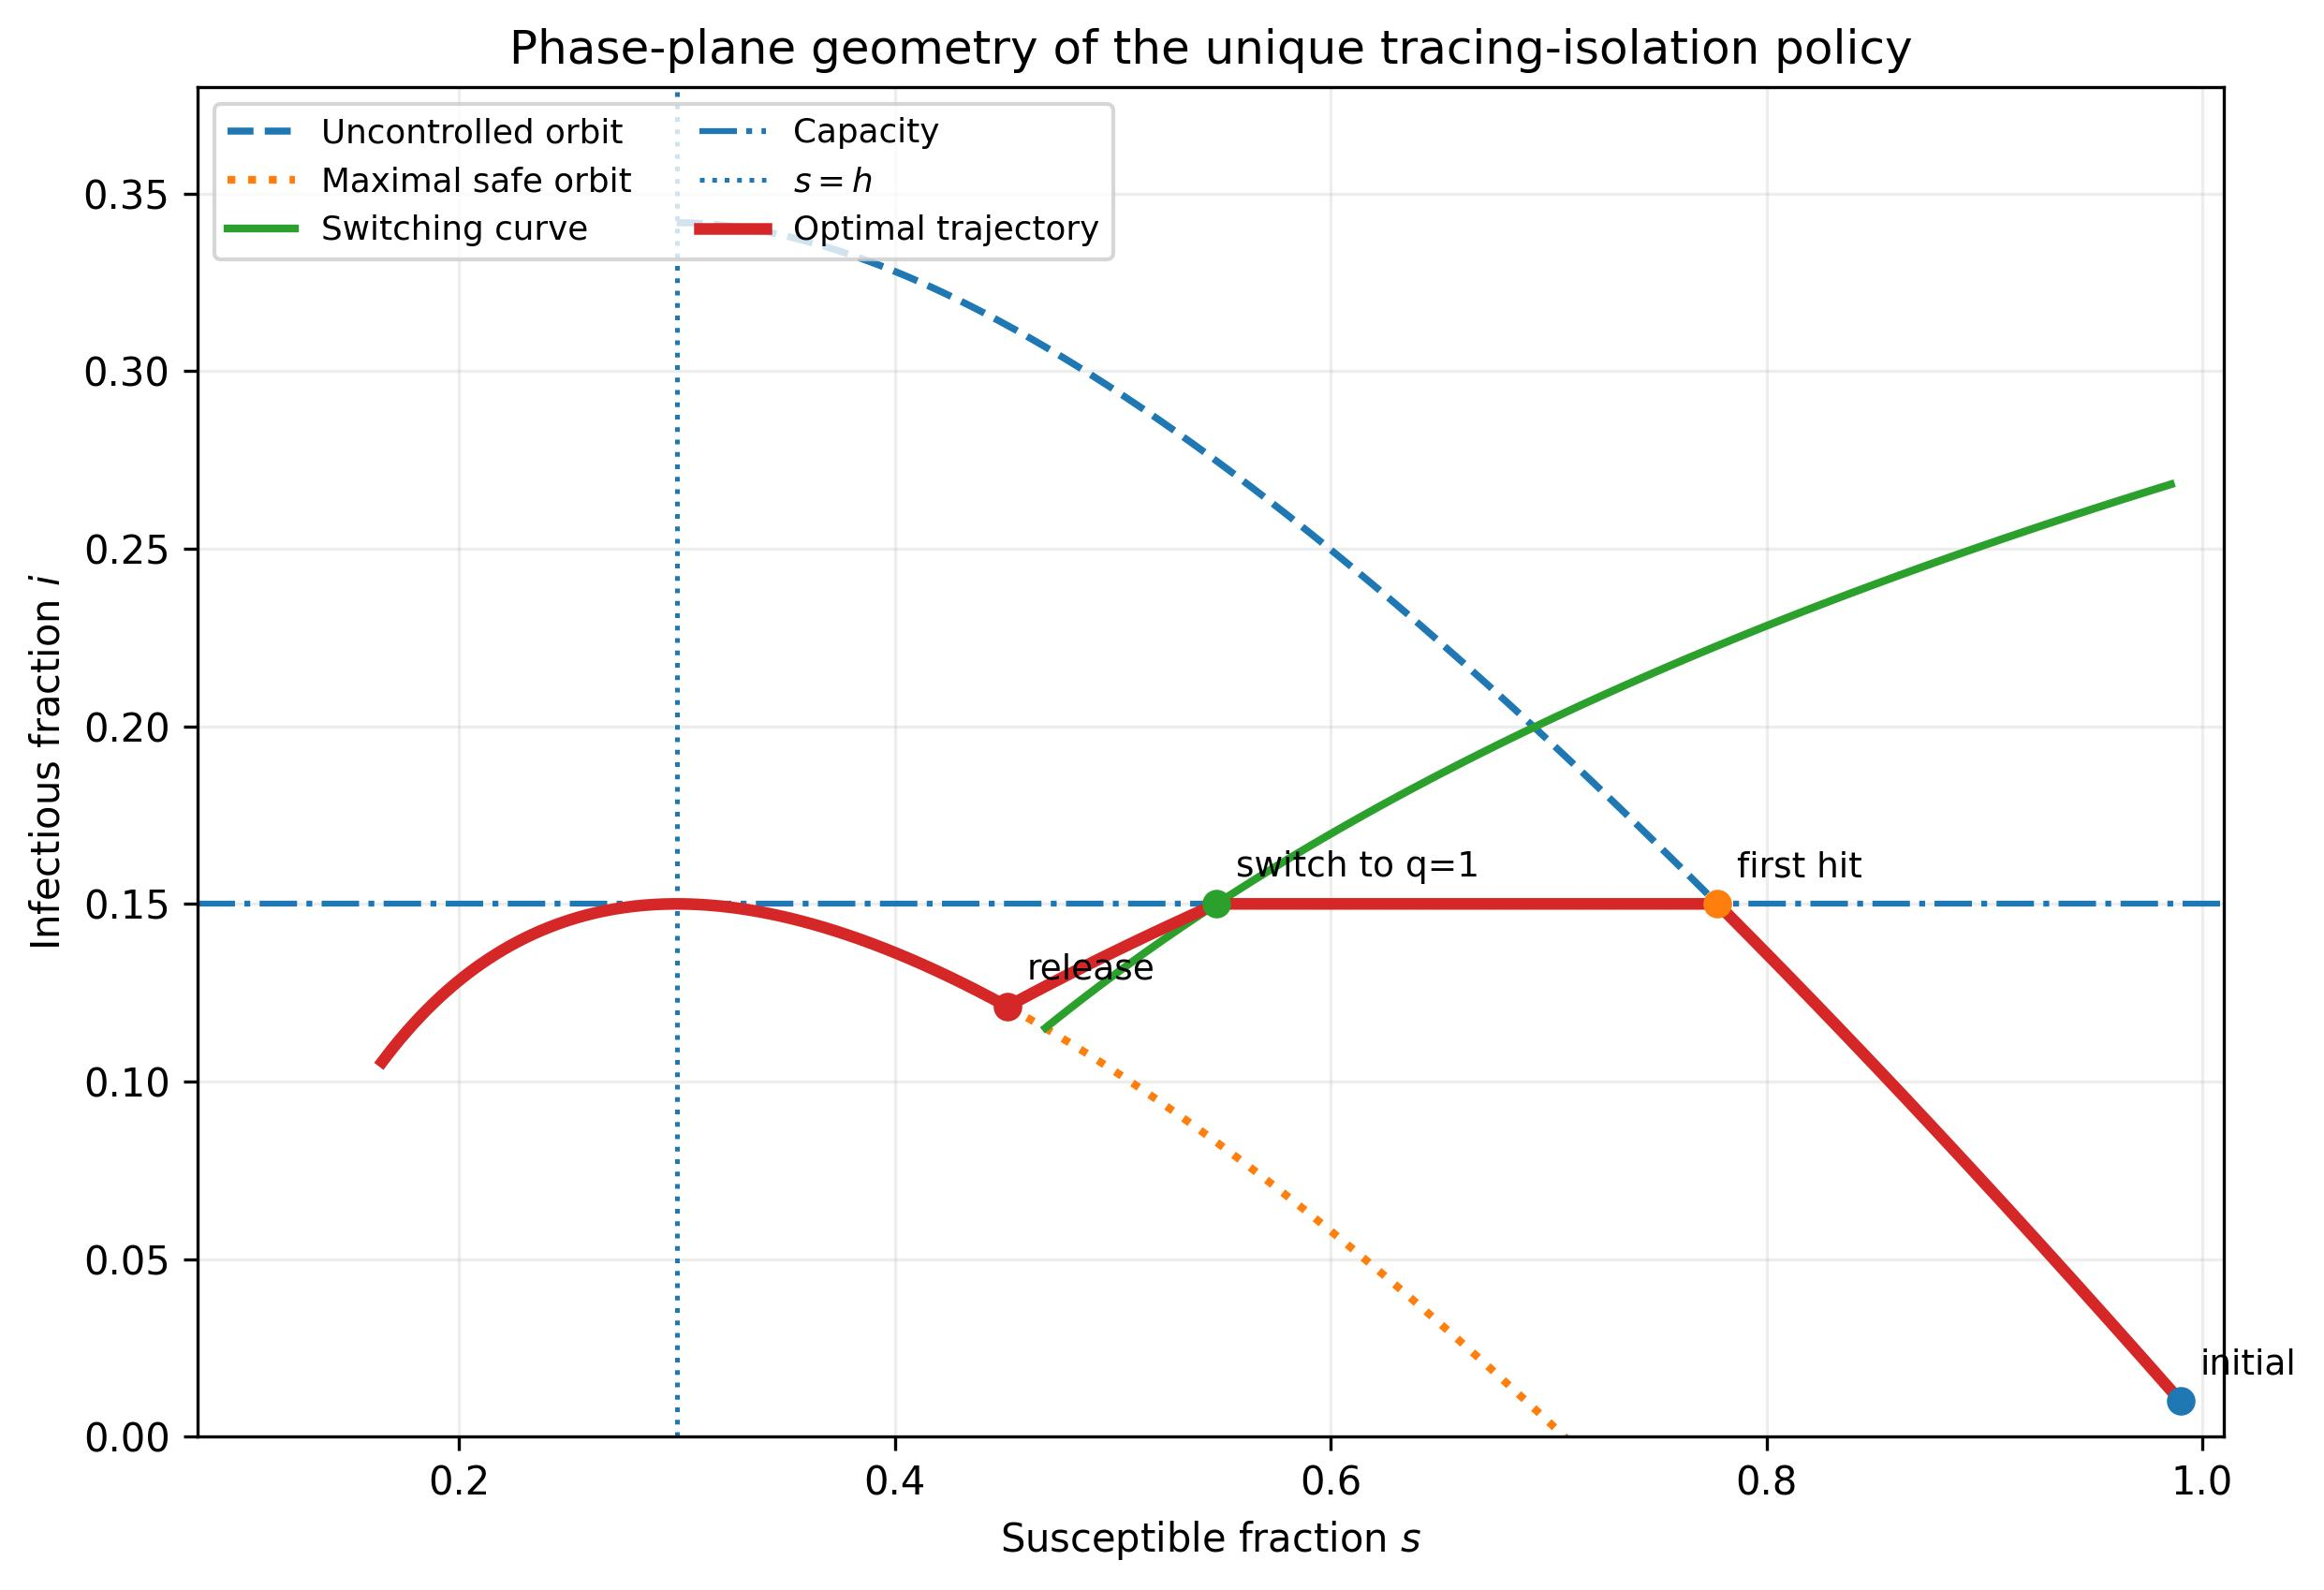
\includegraphics[width=0.94\textwidth]{Figure_1_phase_geometry.jpg}
\caption{常接触率下的相平面几何。虚线为无隔离轨道，点线为最大安全轨道，实细线为切换曲线，粗线为最优轨道。最优轨道先自然到达容量，沿 $i=K$ 运行，再转入 $q=1$，最后在安全边界解除隔离。}
\label{fig:phase}\end{figure}
切换曲线不是容量线或群体免疫直线 $s=h$。
本模型允许在容量边界尚未走到 $h$ 以前转入完全跟踪，这是相对于经典 filling-the-box 的新增结构。

\subsection{状态时间序列}
\begin{figure}[H]\centering

\includegraphics[width=0.92\textwidth]{Figure_2_state_time_series.jpg}
\caption{最优策略下的状态时间序列。感染比例首次达到 $K$ 后保持一段时间，转入完全跟踪后下降，解除隔离以后沿最大安全轨道自然演化。}
\label{fig:states}\end{figure}
$i(t)$ 在平台阶段等于 $K$，完全跟踪后下降到 $i_R<K$。
解除点位于安全边界，后续自然演化可以再次上升至 $K$，但不会超过容量。

\subsection{一个控制产生两个不同系数}
\begin{figure}[H]\centering
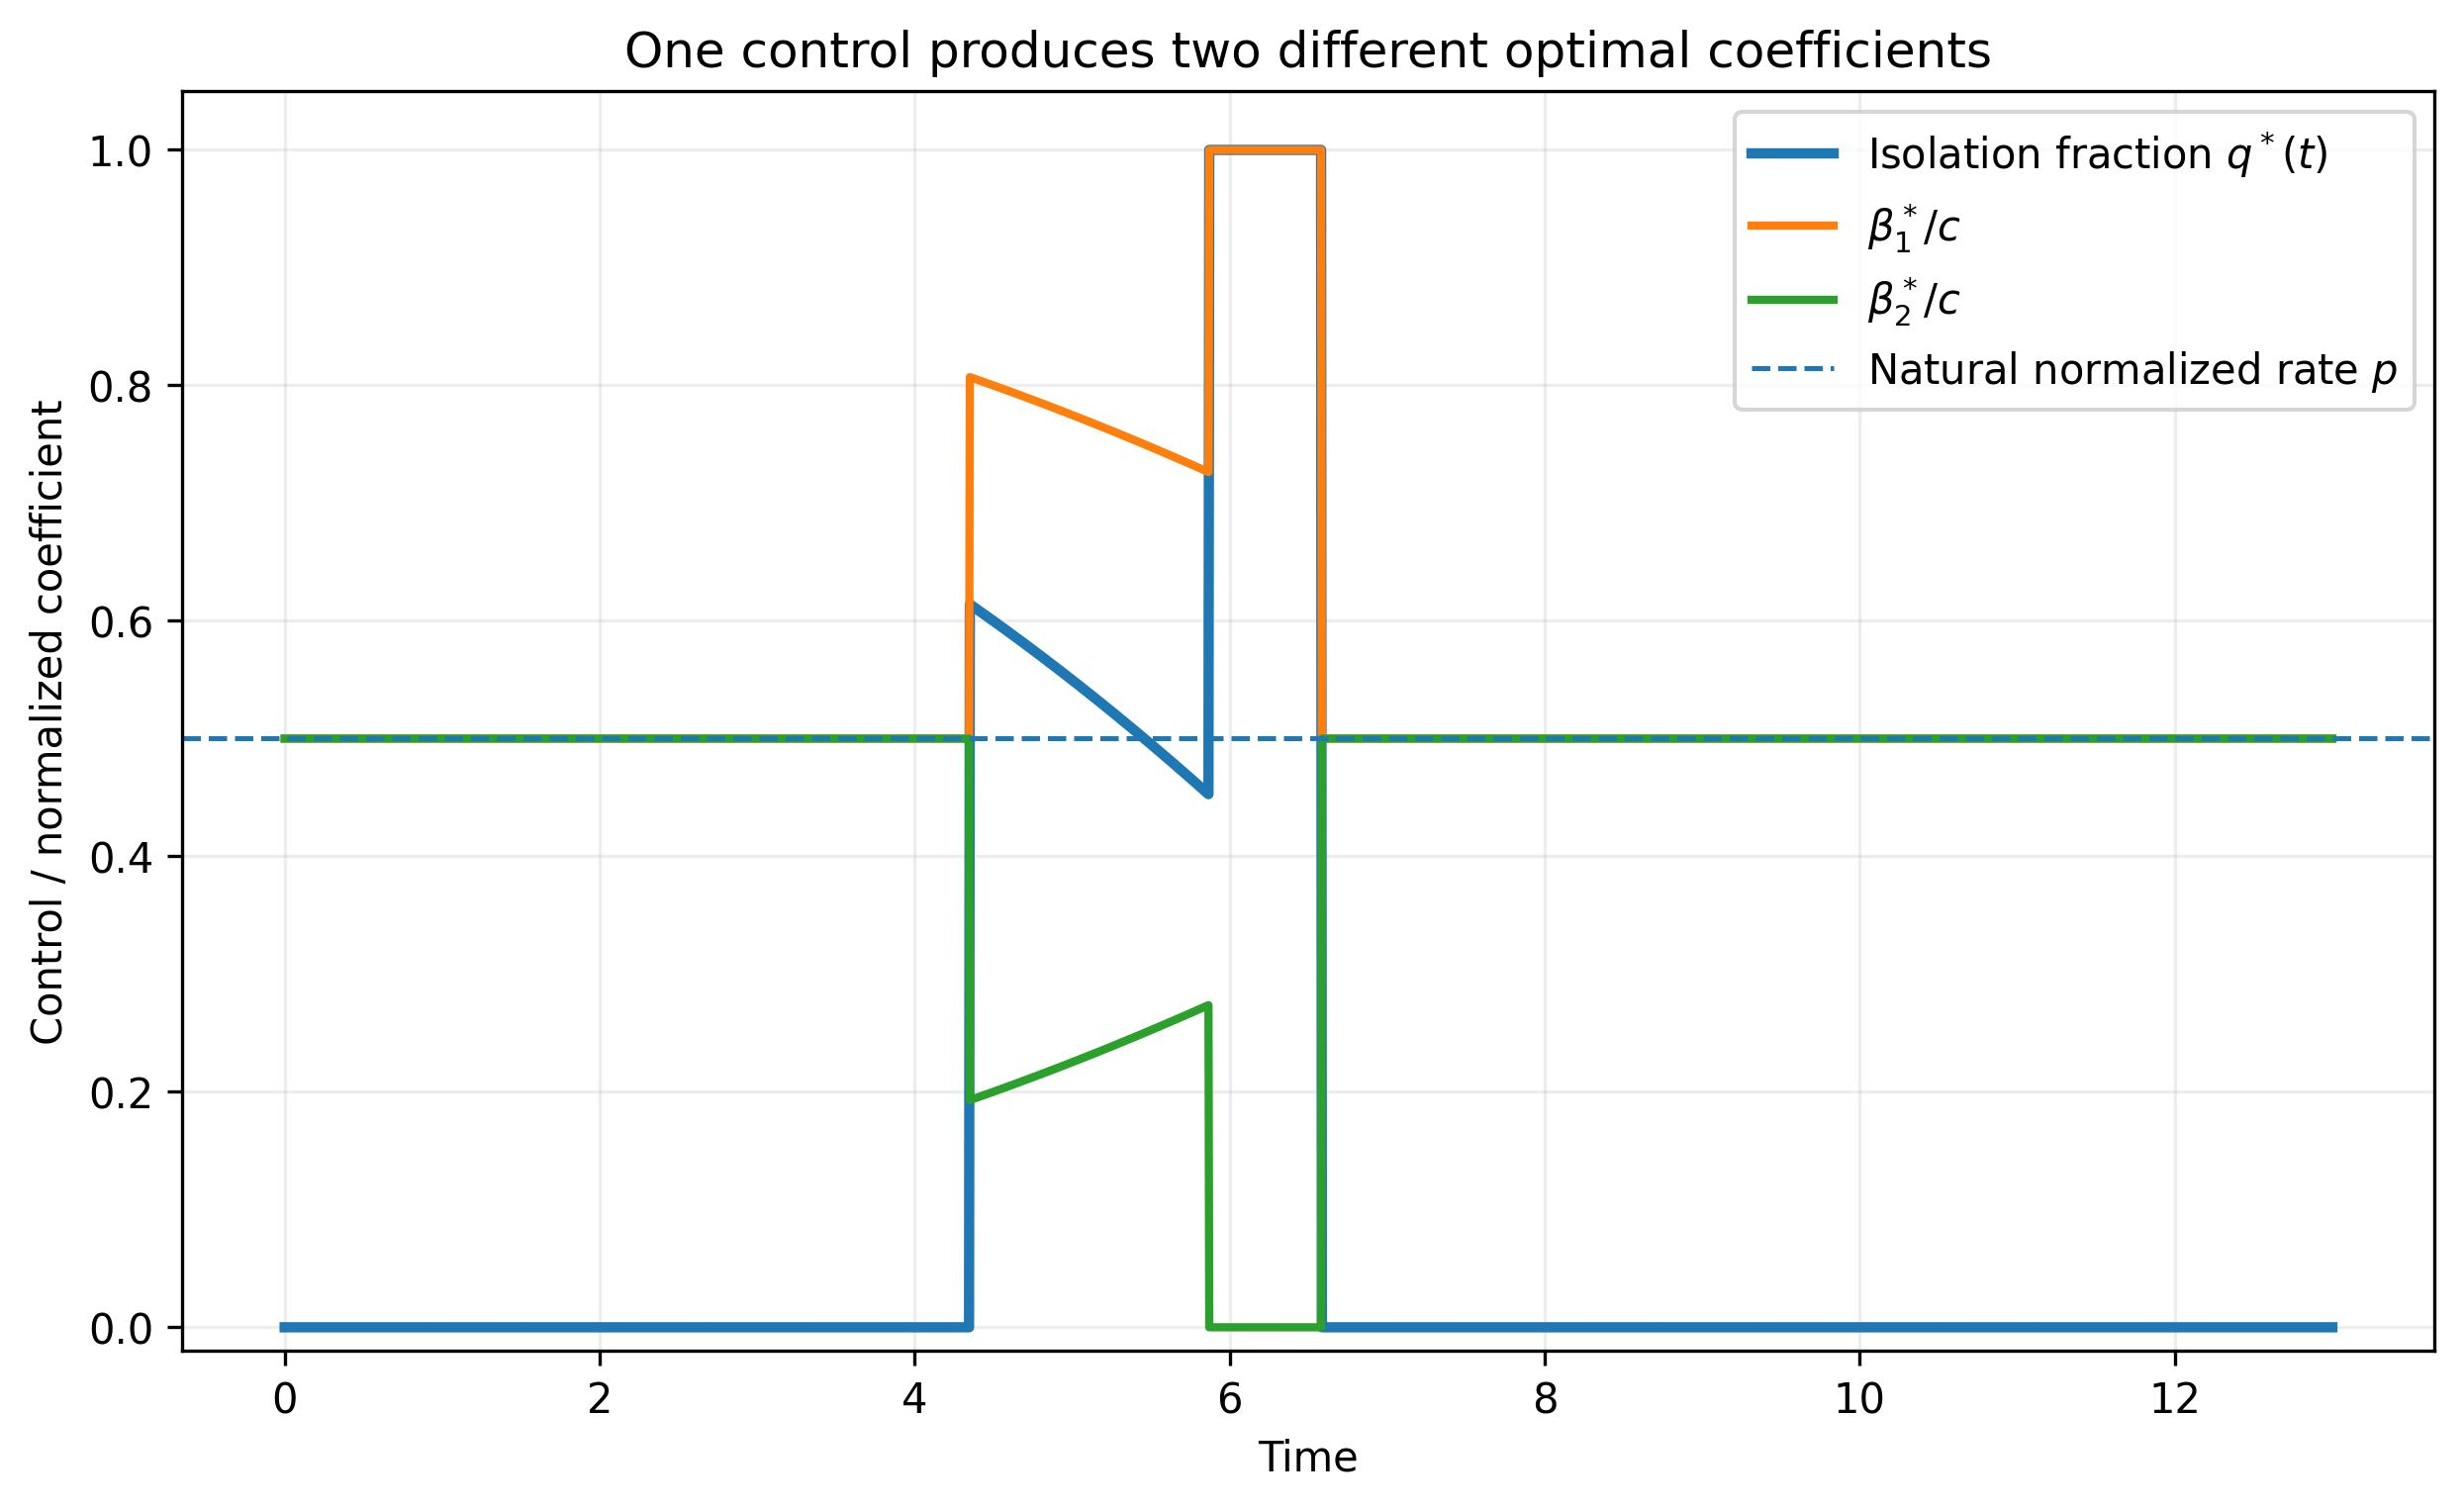
\includegraphics[width=0.92\textwidth]{Figure_3_control_coefficients.jpg}
\caption{最优控制与归一化传播系数。按计数变量记号，应读作 $N\beta_1/c=p+(1-p)q$ 与 $N\beta_2/c=p(1-q)$；前者随 $q$ 上升，后者随 $q$ 下降。}
\label{fig:coefficients}\end{figure}
平台控制 $q_B=1-h/s$ 随 $s$ 下降而下降；完全跟踪 $q=1$ 时，$\beta_2=0$，感染按恢复率衰减。

\subsection{一维成本曲线的数值展示}
\begin{figure}[H]\centering
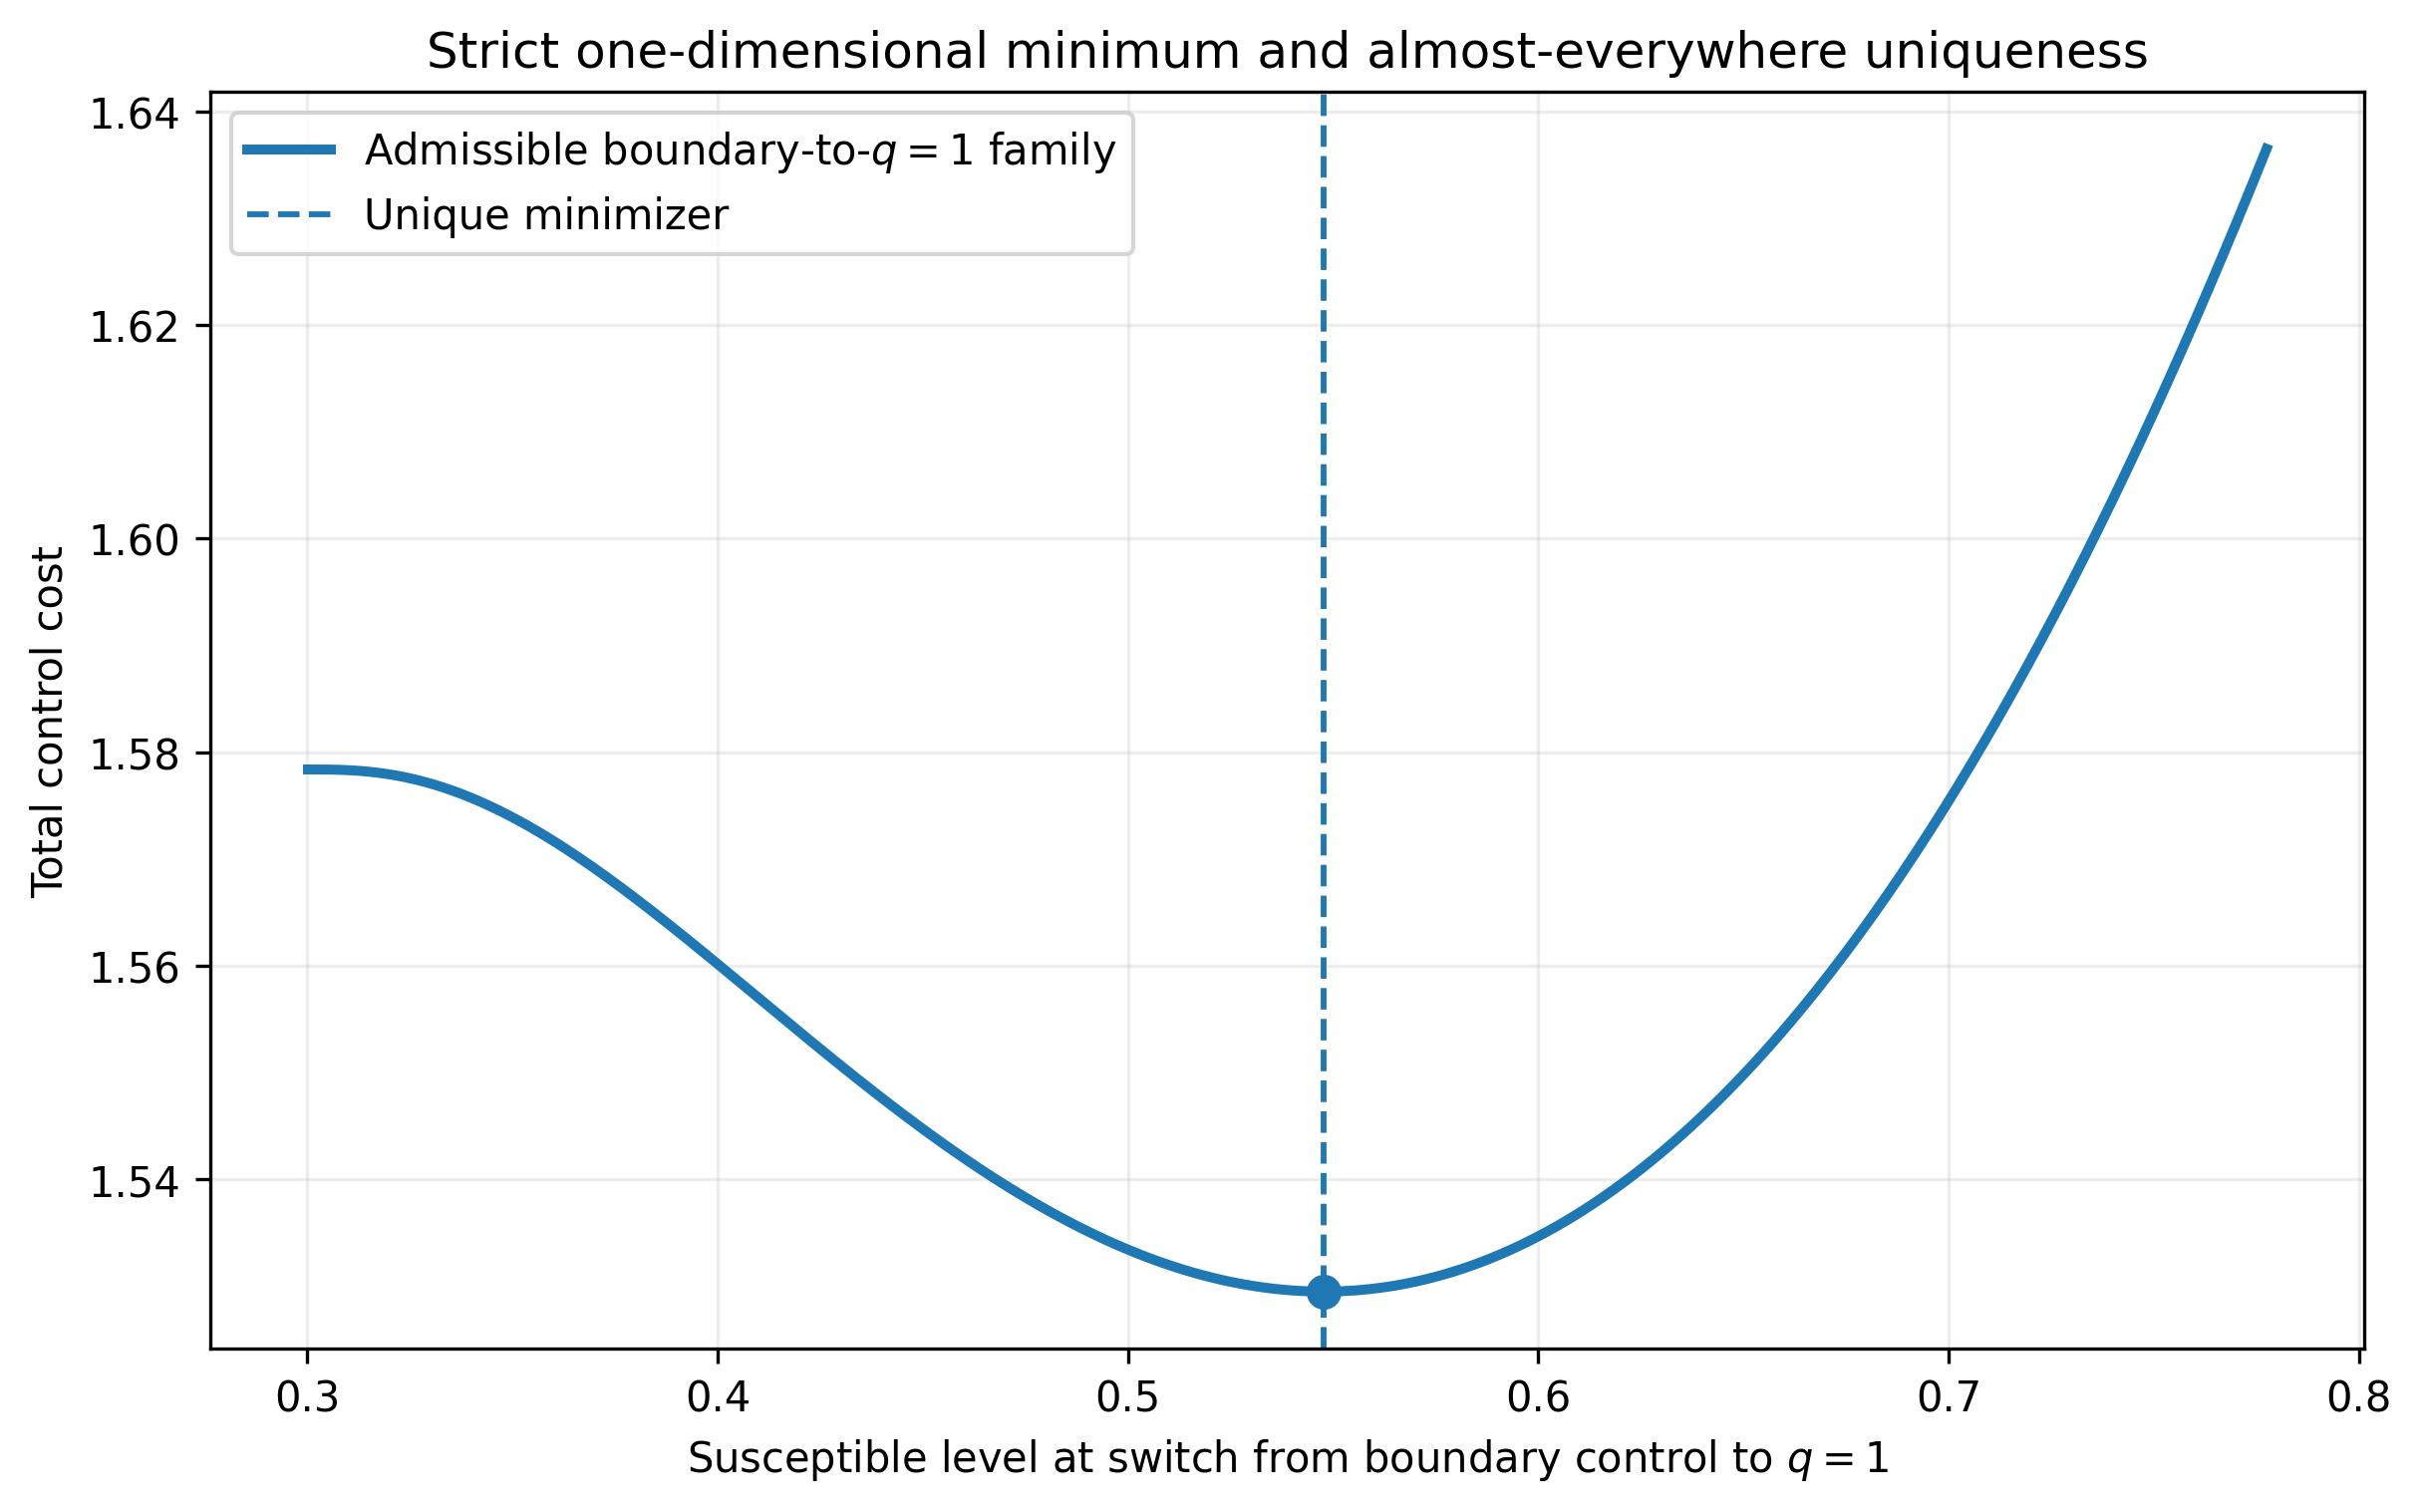
\includegraphics[width=0.9\textwidth]{Figure_4_uniqueness_cost.jpg}
\caption{容量转完全跟踪位置与总成本的关系。曲线展示一维策略族的严格极小；解析依据为 \eqref{eq:JB-derivative} 及推论\ref{cor:one-dimensional-min}，图形本身不承担全局最优性证明。}
\label{fig:unique-cost}\end{figure}
该曲线由容量成本与完全跟踪成本相加得到；所有可测控制之间的比较由全域验证定理完成。

\subsection{可行策略成本比较}
\begin{figure}[H]\centering
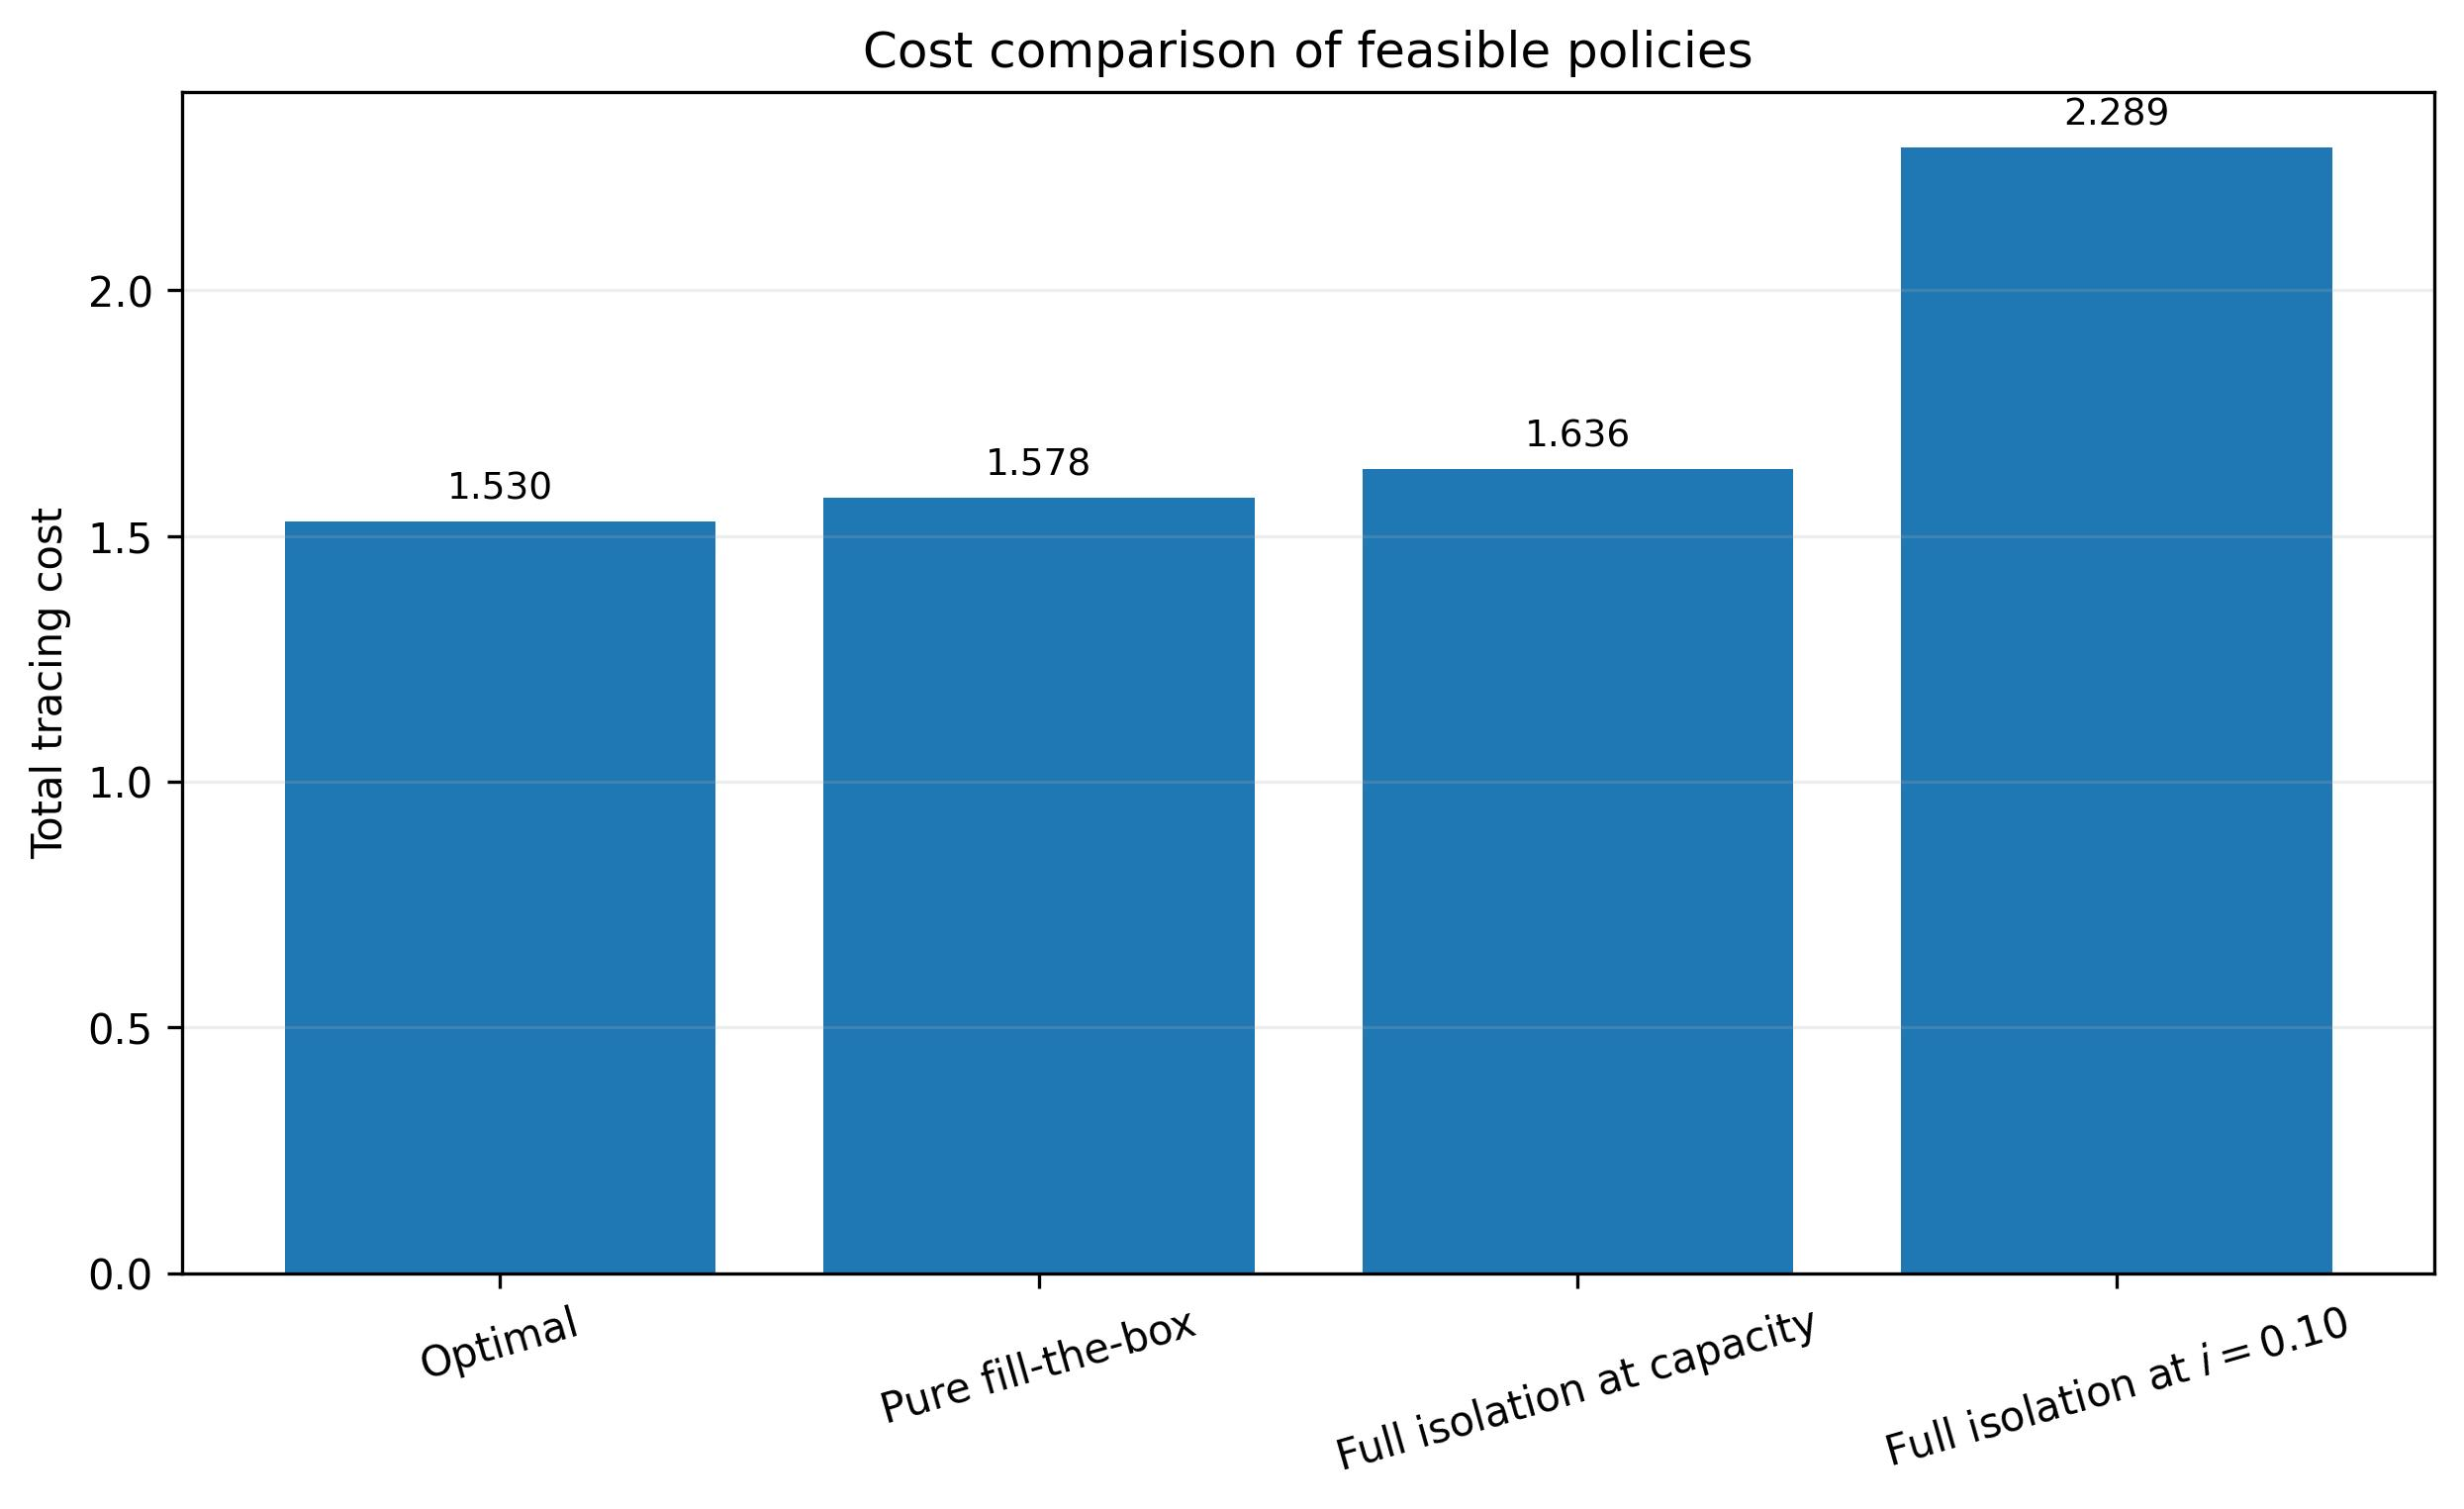
\includegraphics[width=0.9\textwidth]{Figure_5_policy_cost_comparison.jpg}
\caption{基准参数下四种可行策略的成本比较。容量边界--完全跟踪组合低于纯容量填充、到容量即完全跟踪和所展示的更早完全跟踪方案。}
\label{fig:policy-cost}\end{figure}

\subsection{容量、传播概率与结构区间}
\begin{figure}[H]\centering
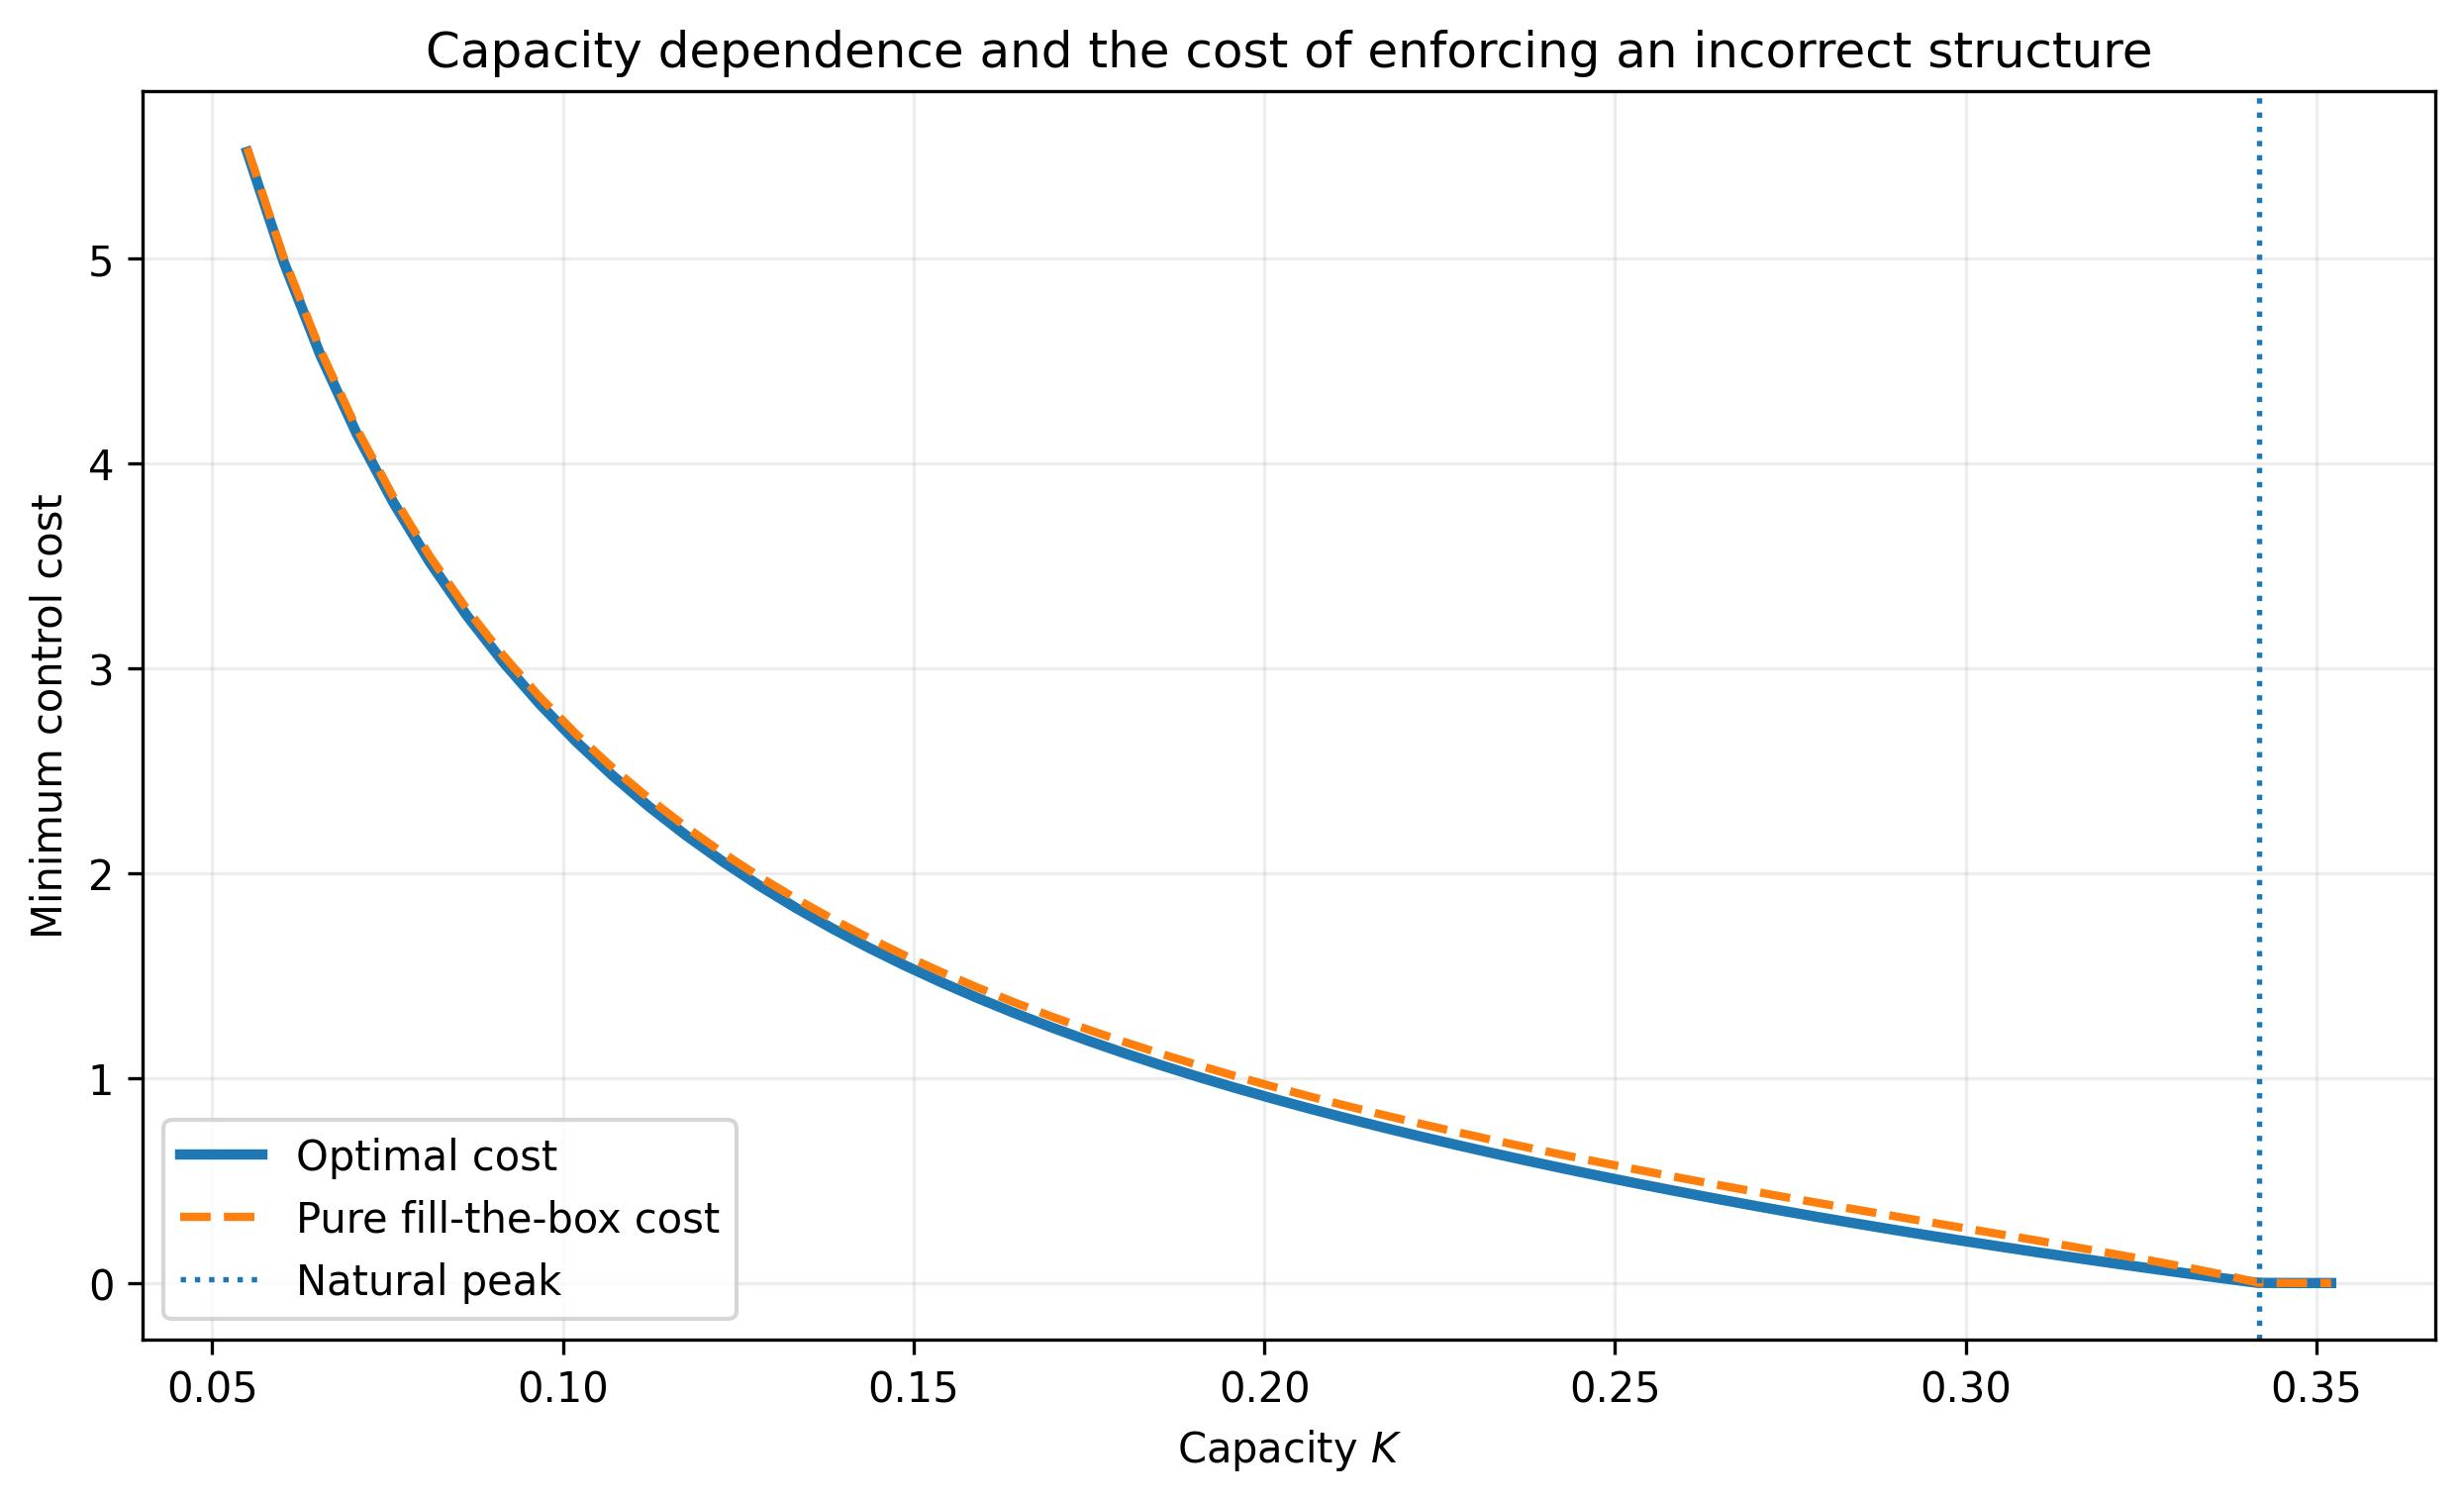
\includegraphics[width=0.9\textwidth]{Figure_6_capacity_dependence.jpg}
\caption{最小成本随医疗容量变化的数值评价。容量增大时可行控制类扩大，所以值函数不增；自然传播安全时成本为零。}
\label{fig:capacity}\end{figure}
\begin{figure}[H]\centering
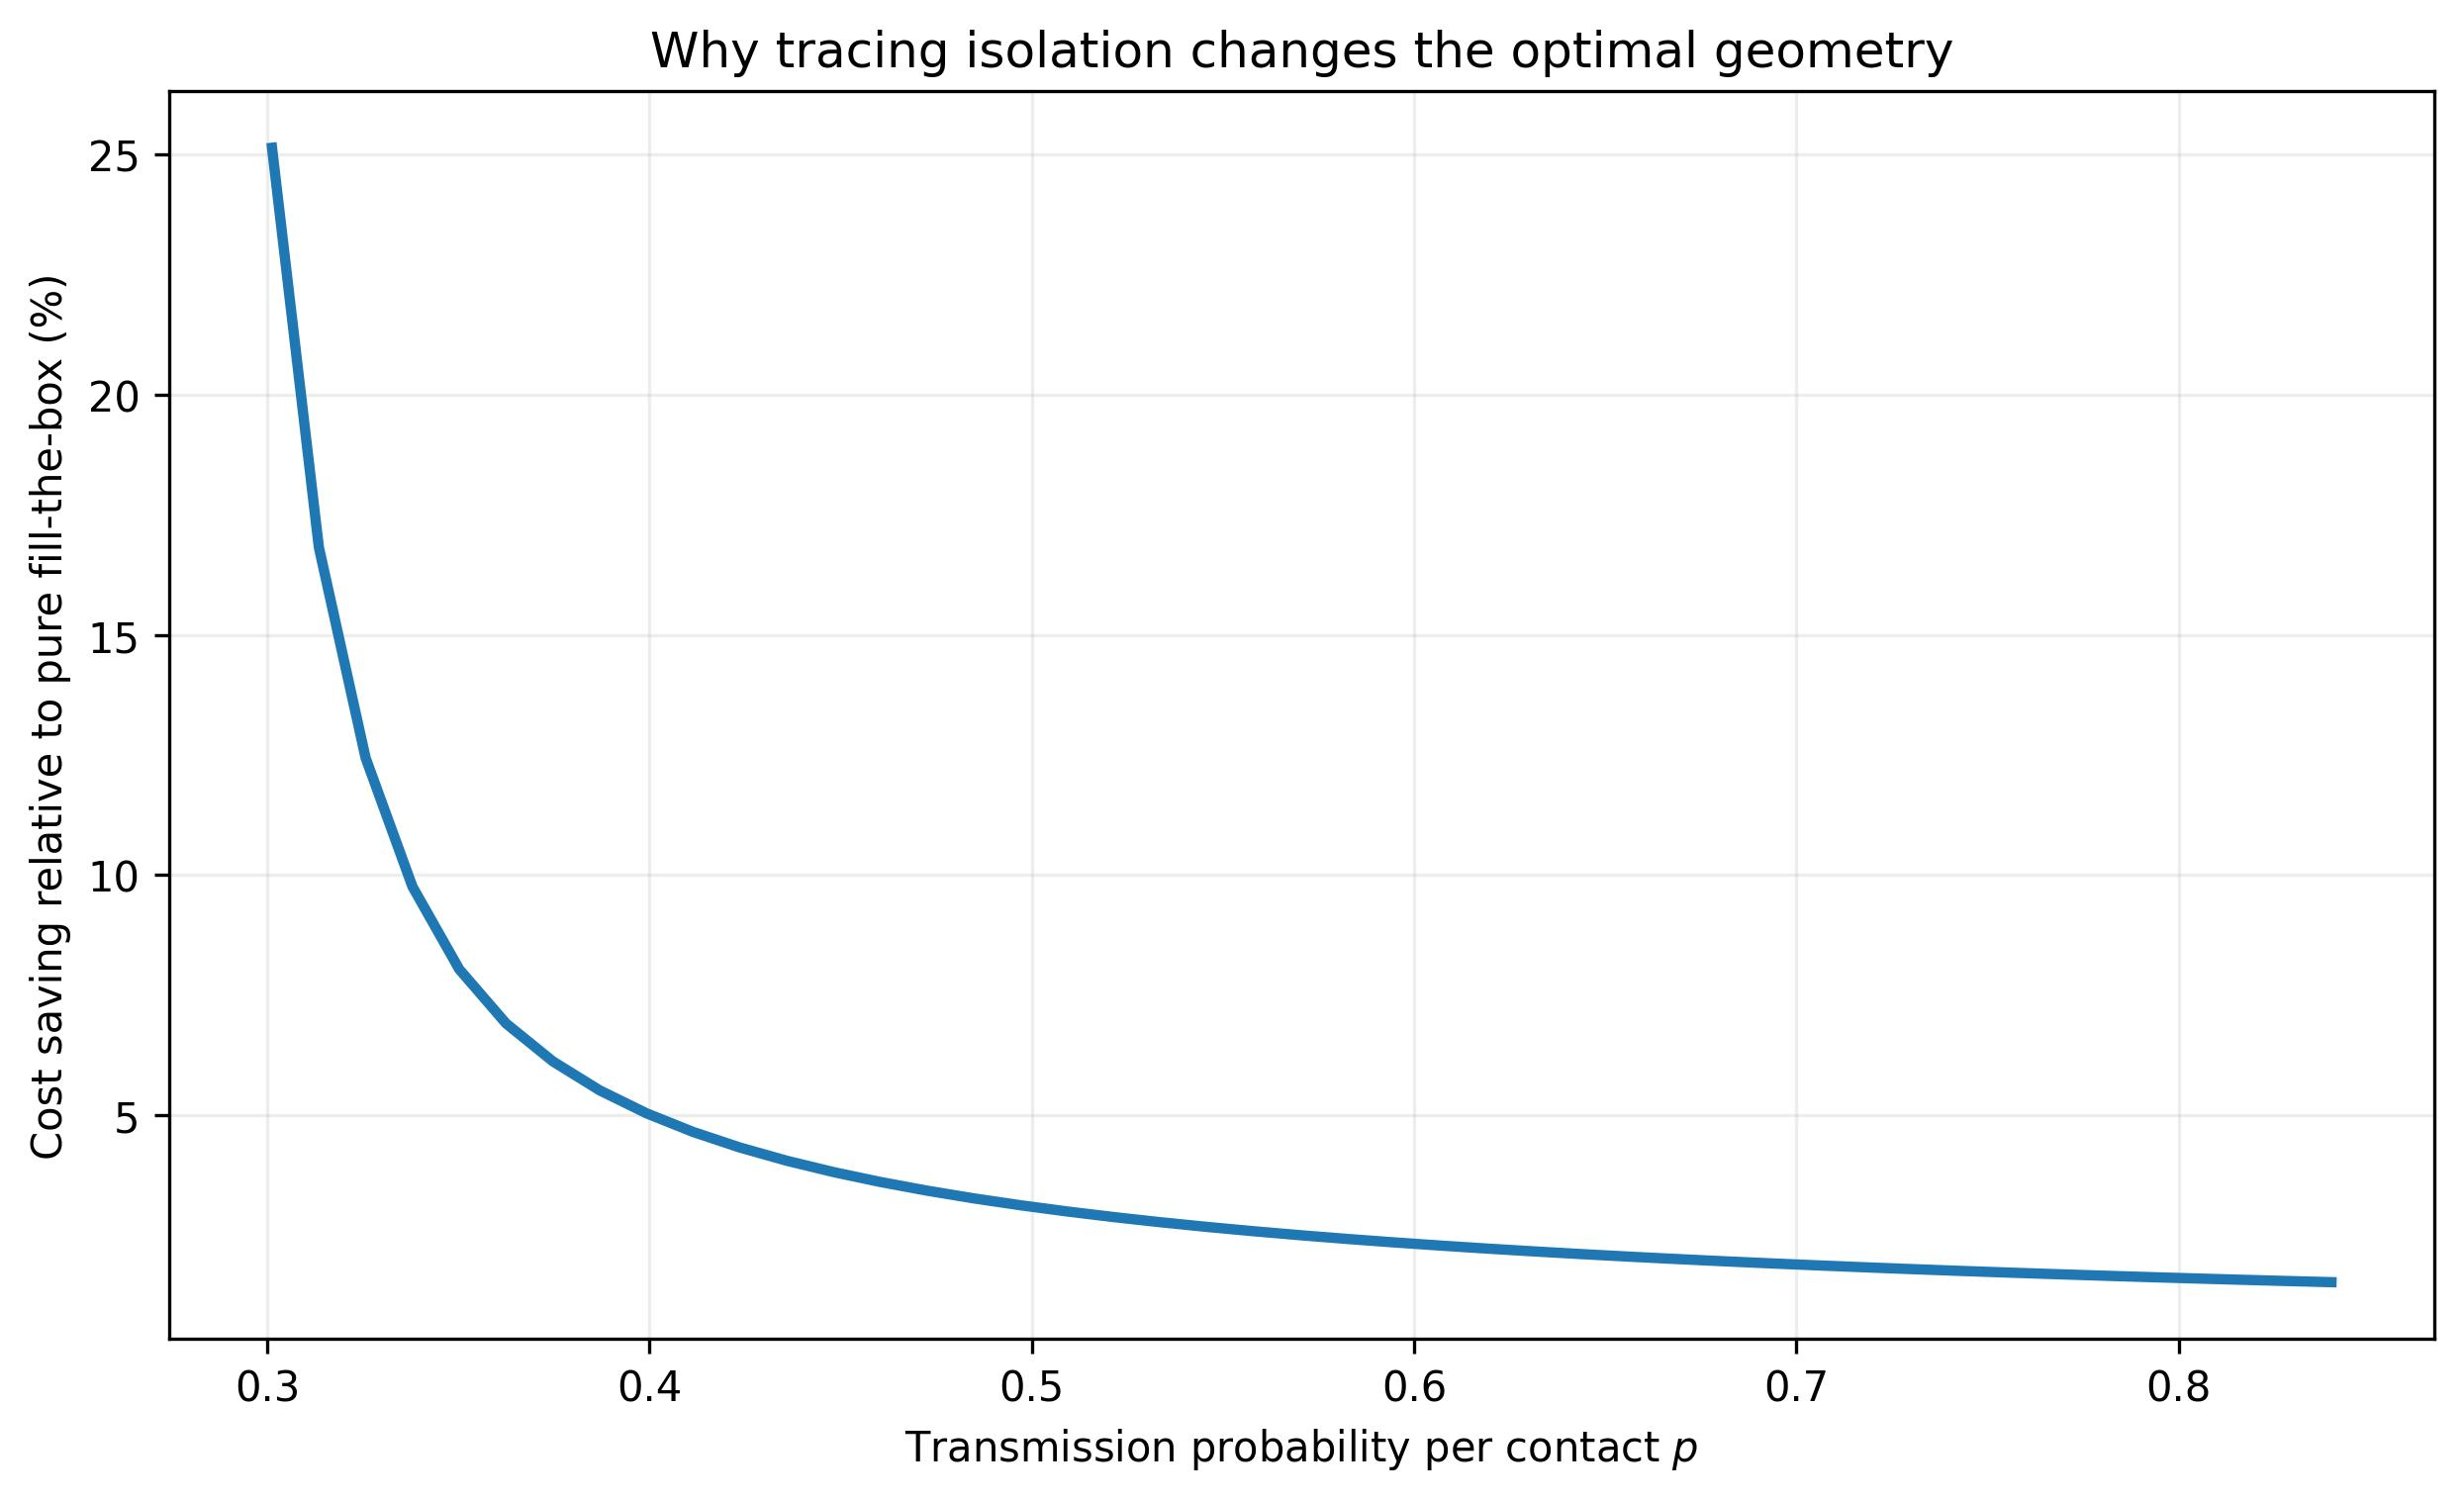
\includegraphics[width=0.9\textwidth]{Figure_7_probability_dependence.jpg}
\caption{原工程参数扫描中，相对于纯容量填充的成本节省随传播概率变化的数值结果。该图不构成对所有参数的严格比较静态结论。}
\label{fig:p-sensitivity}\end{figure}
\begin{figure}[H]\centering
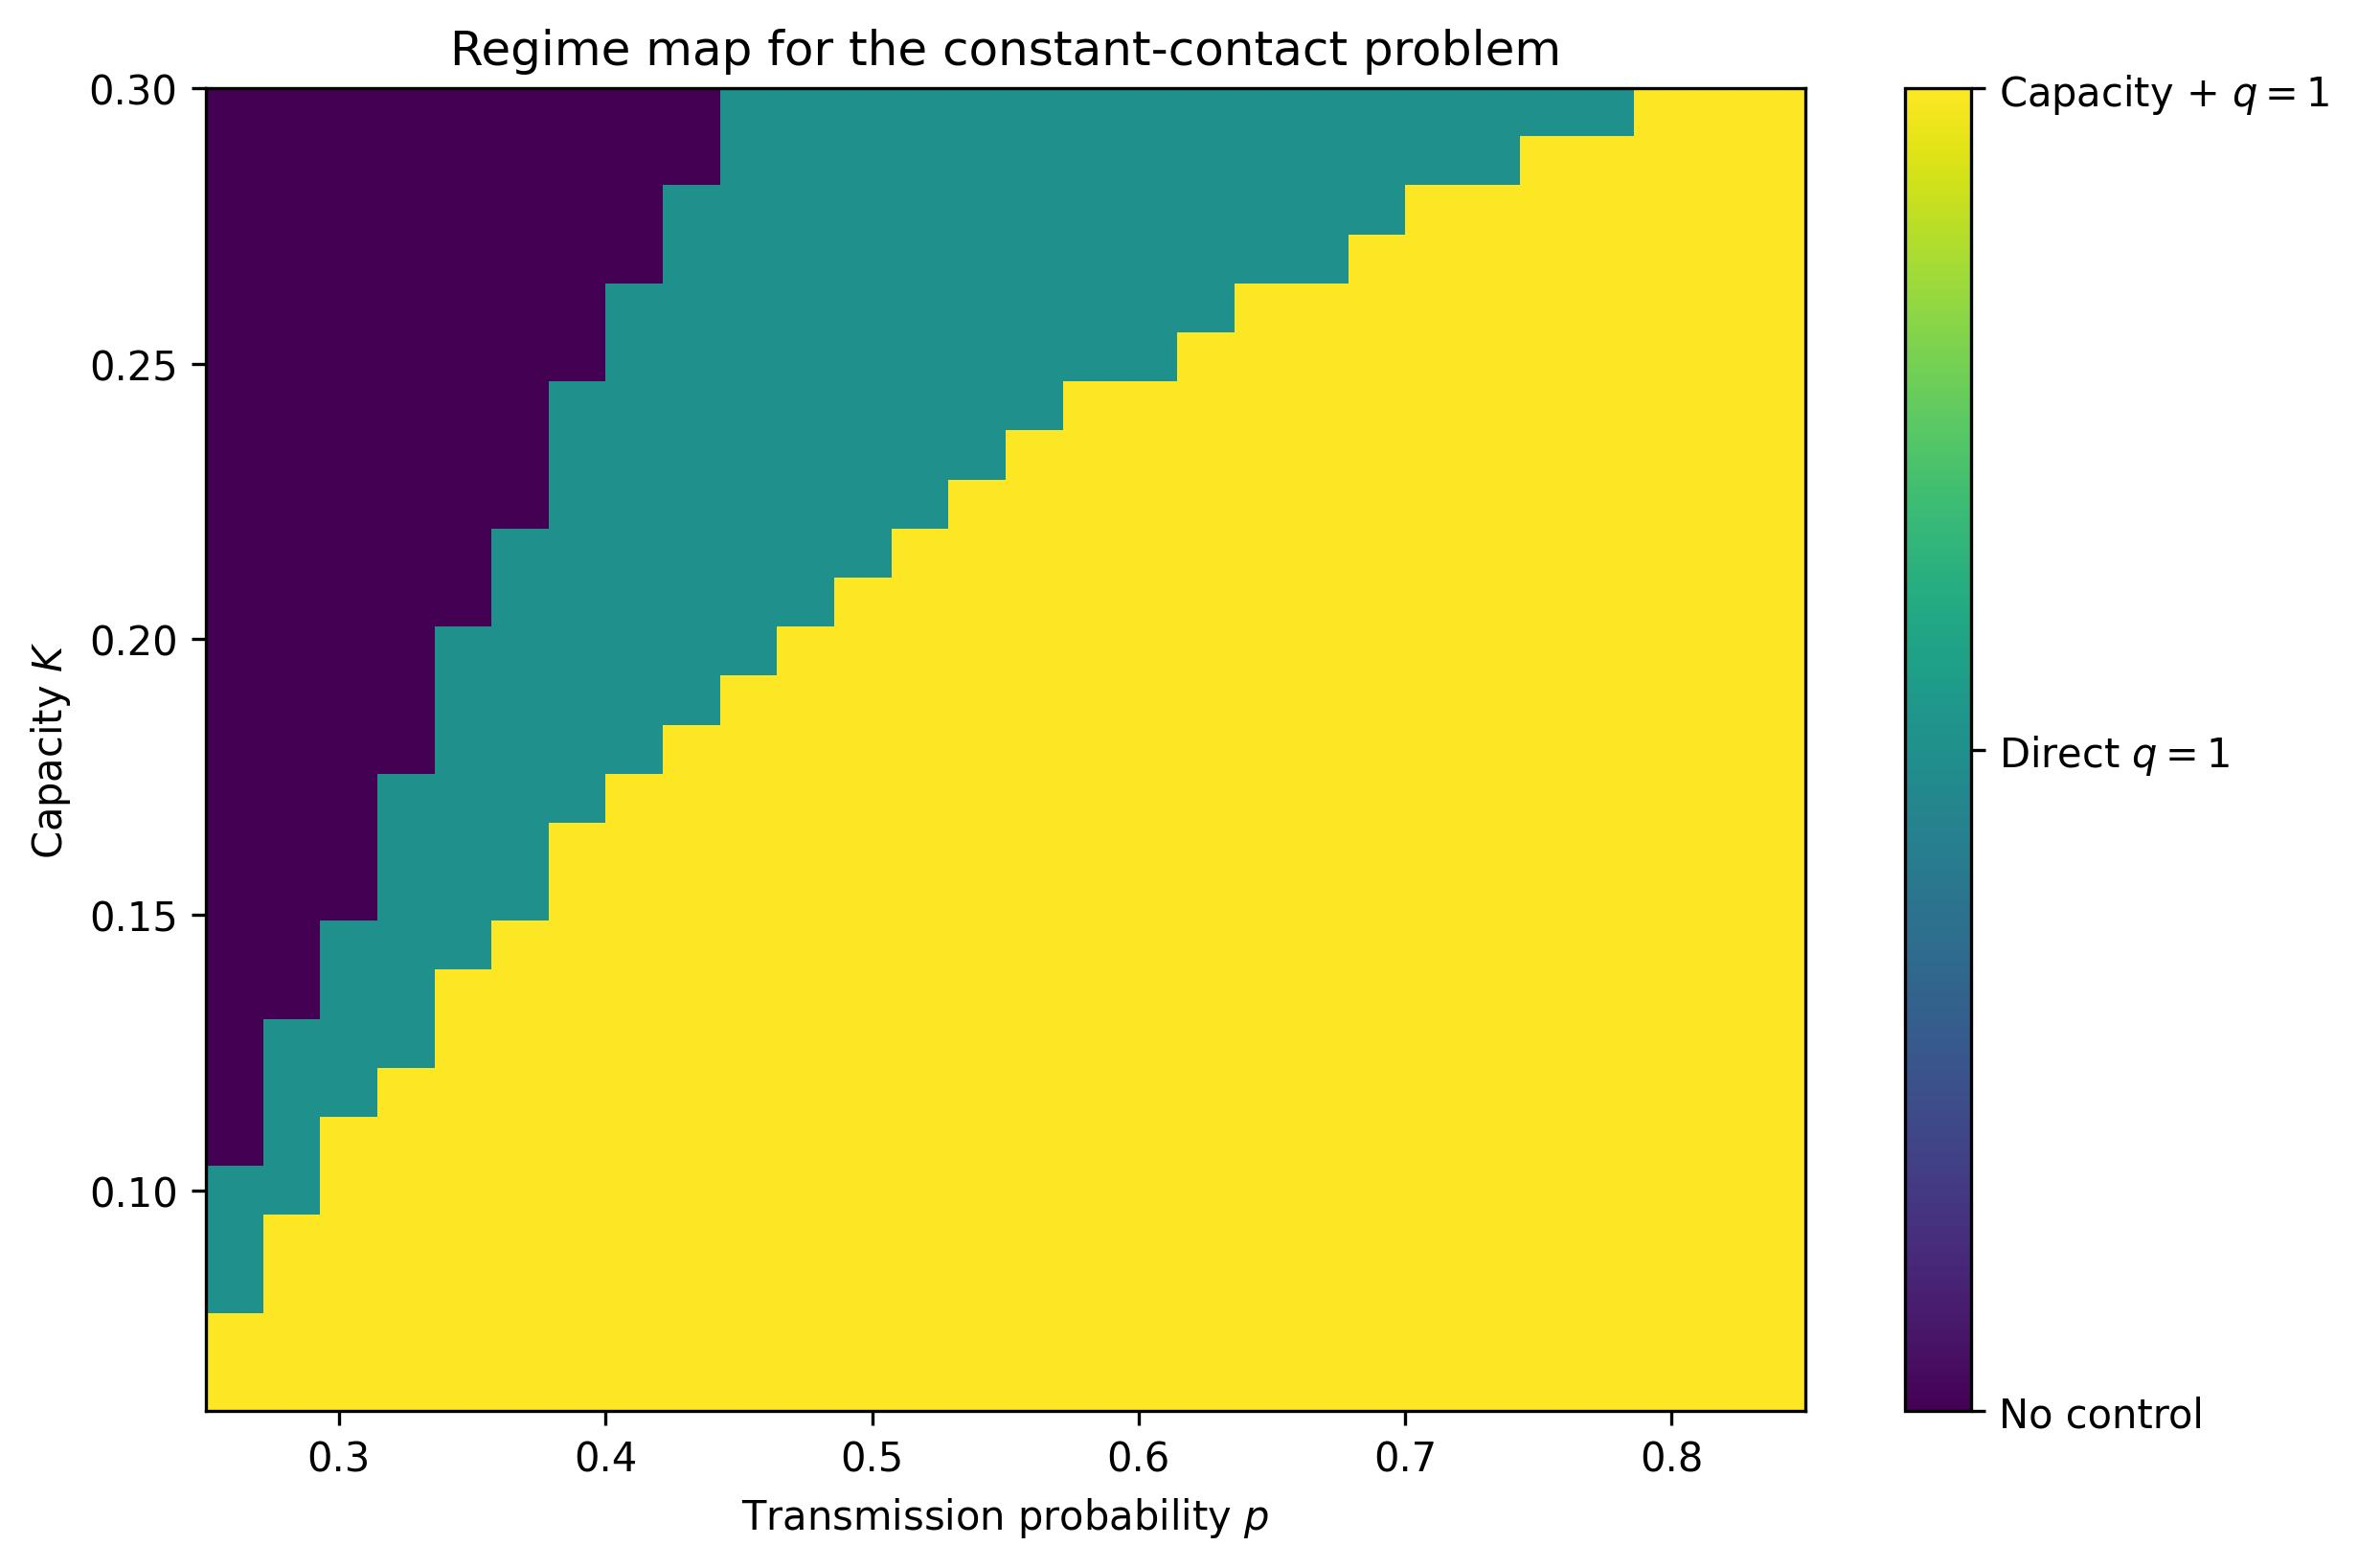
\includegraphics[width=0.9\textwidth]{Figure_8_regime_map.jpg}
\caption{原工程 $p$--$K$ 参数扫描的结构图。一般初值的精确判别应使用定义\ref{def:regions}，并允许初始即处于完全跟踪区。}
\label{fig:regime}\end{figure}
“先到容量”不是所有参数和初值下的共同结构；自然安全、容量前直接跟踪以及正长度容量平台都可能出现。

\subsection{时变接触率的原工程离散结果}
保留原接触高峰函数
\begin{equation}
c(t)=2\left[1+0.55\exp\left(-\frac12\left(\frac{t-5.5}{1.35}\right)^2\right)\right].
\label{eq:contact-surge}
\end{equation}
它在有限时间仍严格大于 $2$，只在无穷远趋于基准值。
\begin{figure}[H]\centering
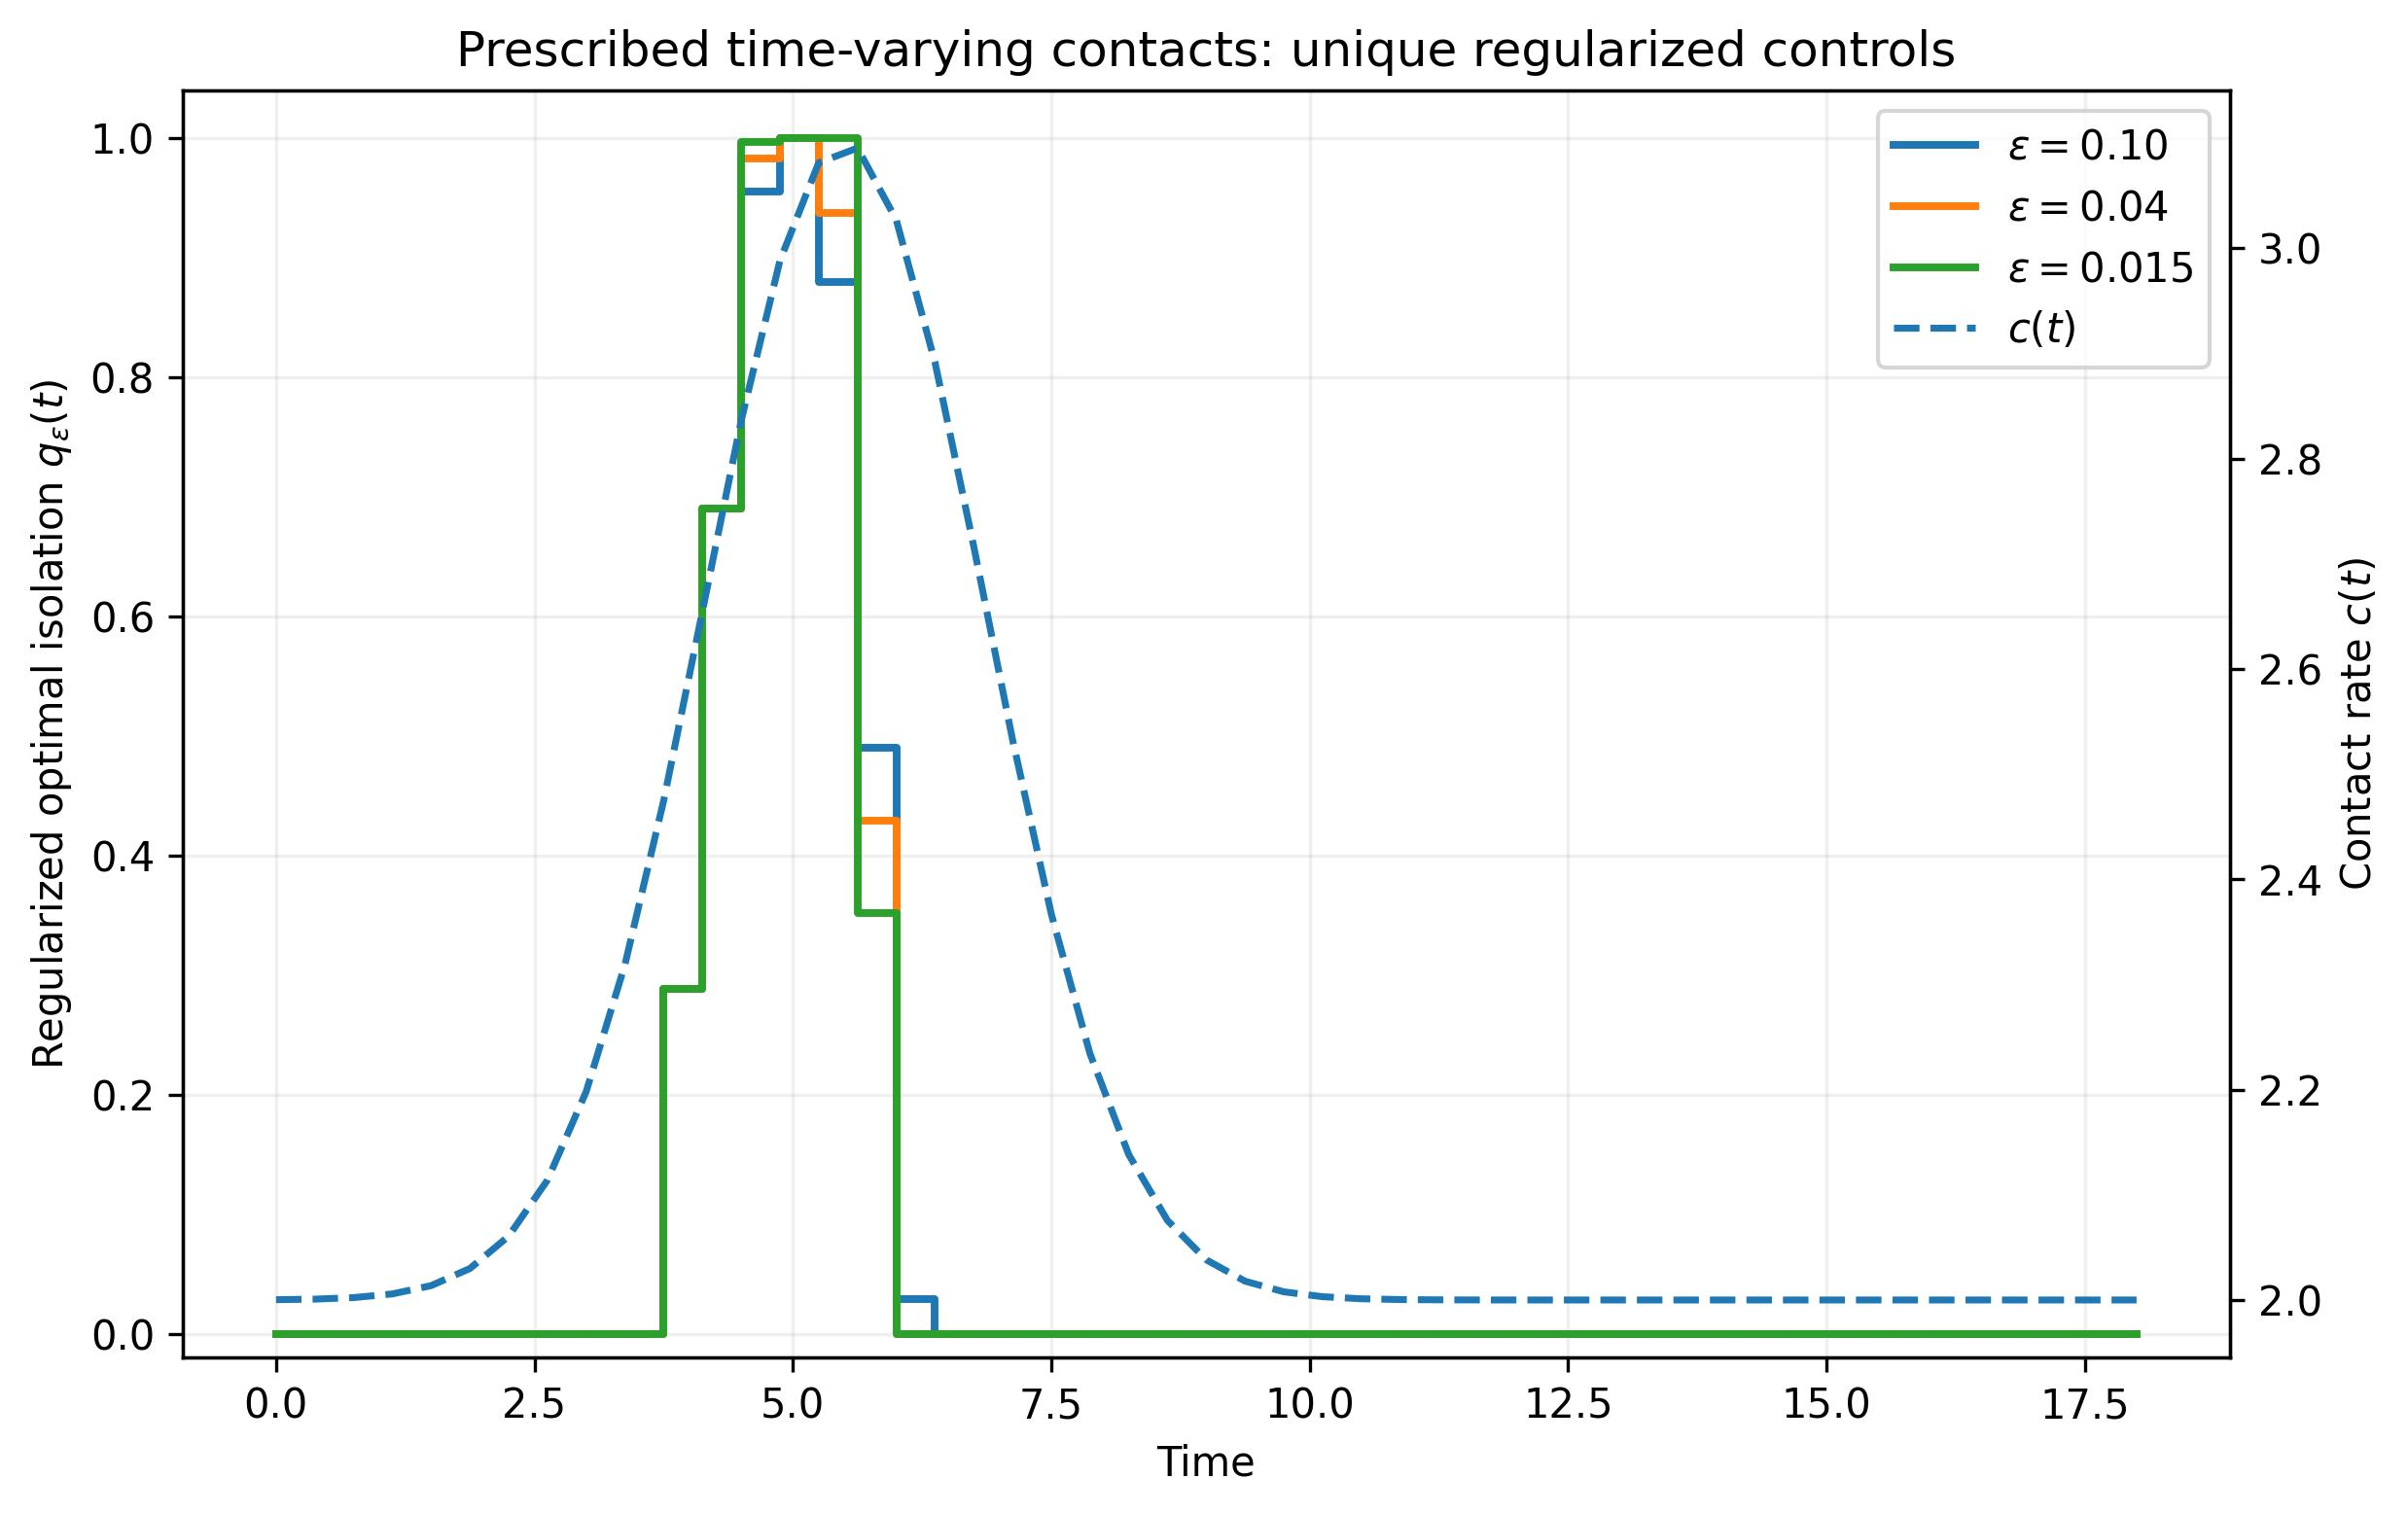
\includegraphics[width=0.92\textwidth]{Figure_9_time_varying_control.jpg}
\caption{给定时变接触率时，不同 $\varepsilon$ 下由原工程离散求解器得到的控制。这里不声称这些离散解全局唯一，也未证明 $\varepsilon\downarrow0$ 时收敛到原连续问题的最优控制。}
\label{fig:time-control}\end{figure}
\begin{figure}[H]\centering
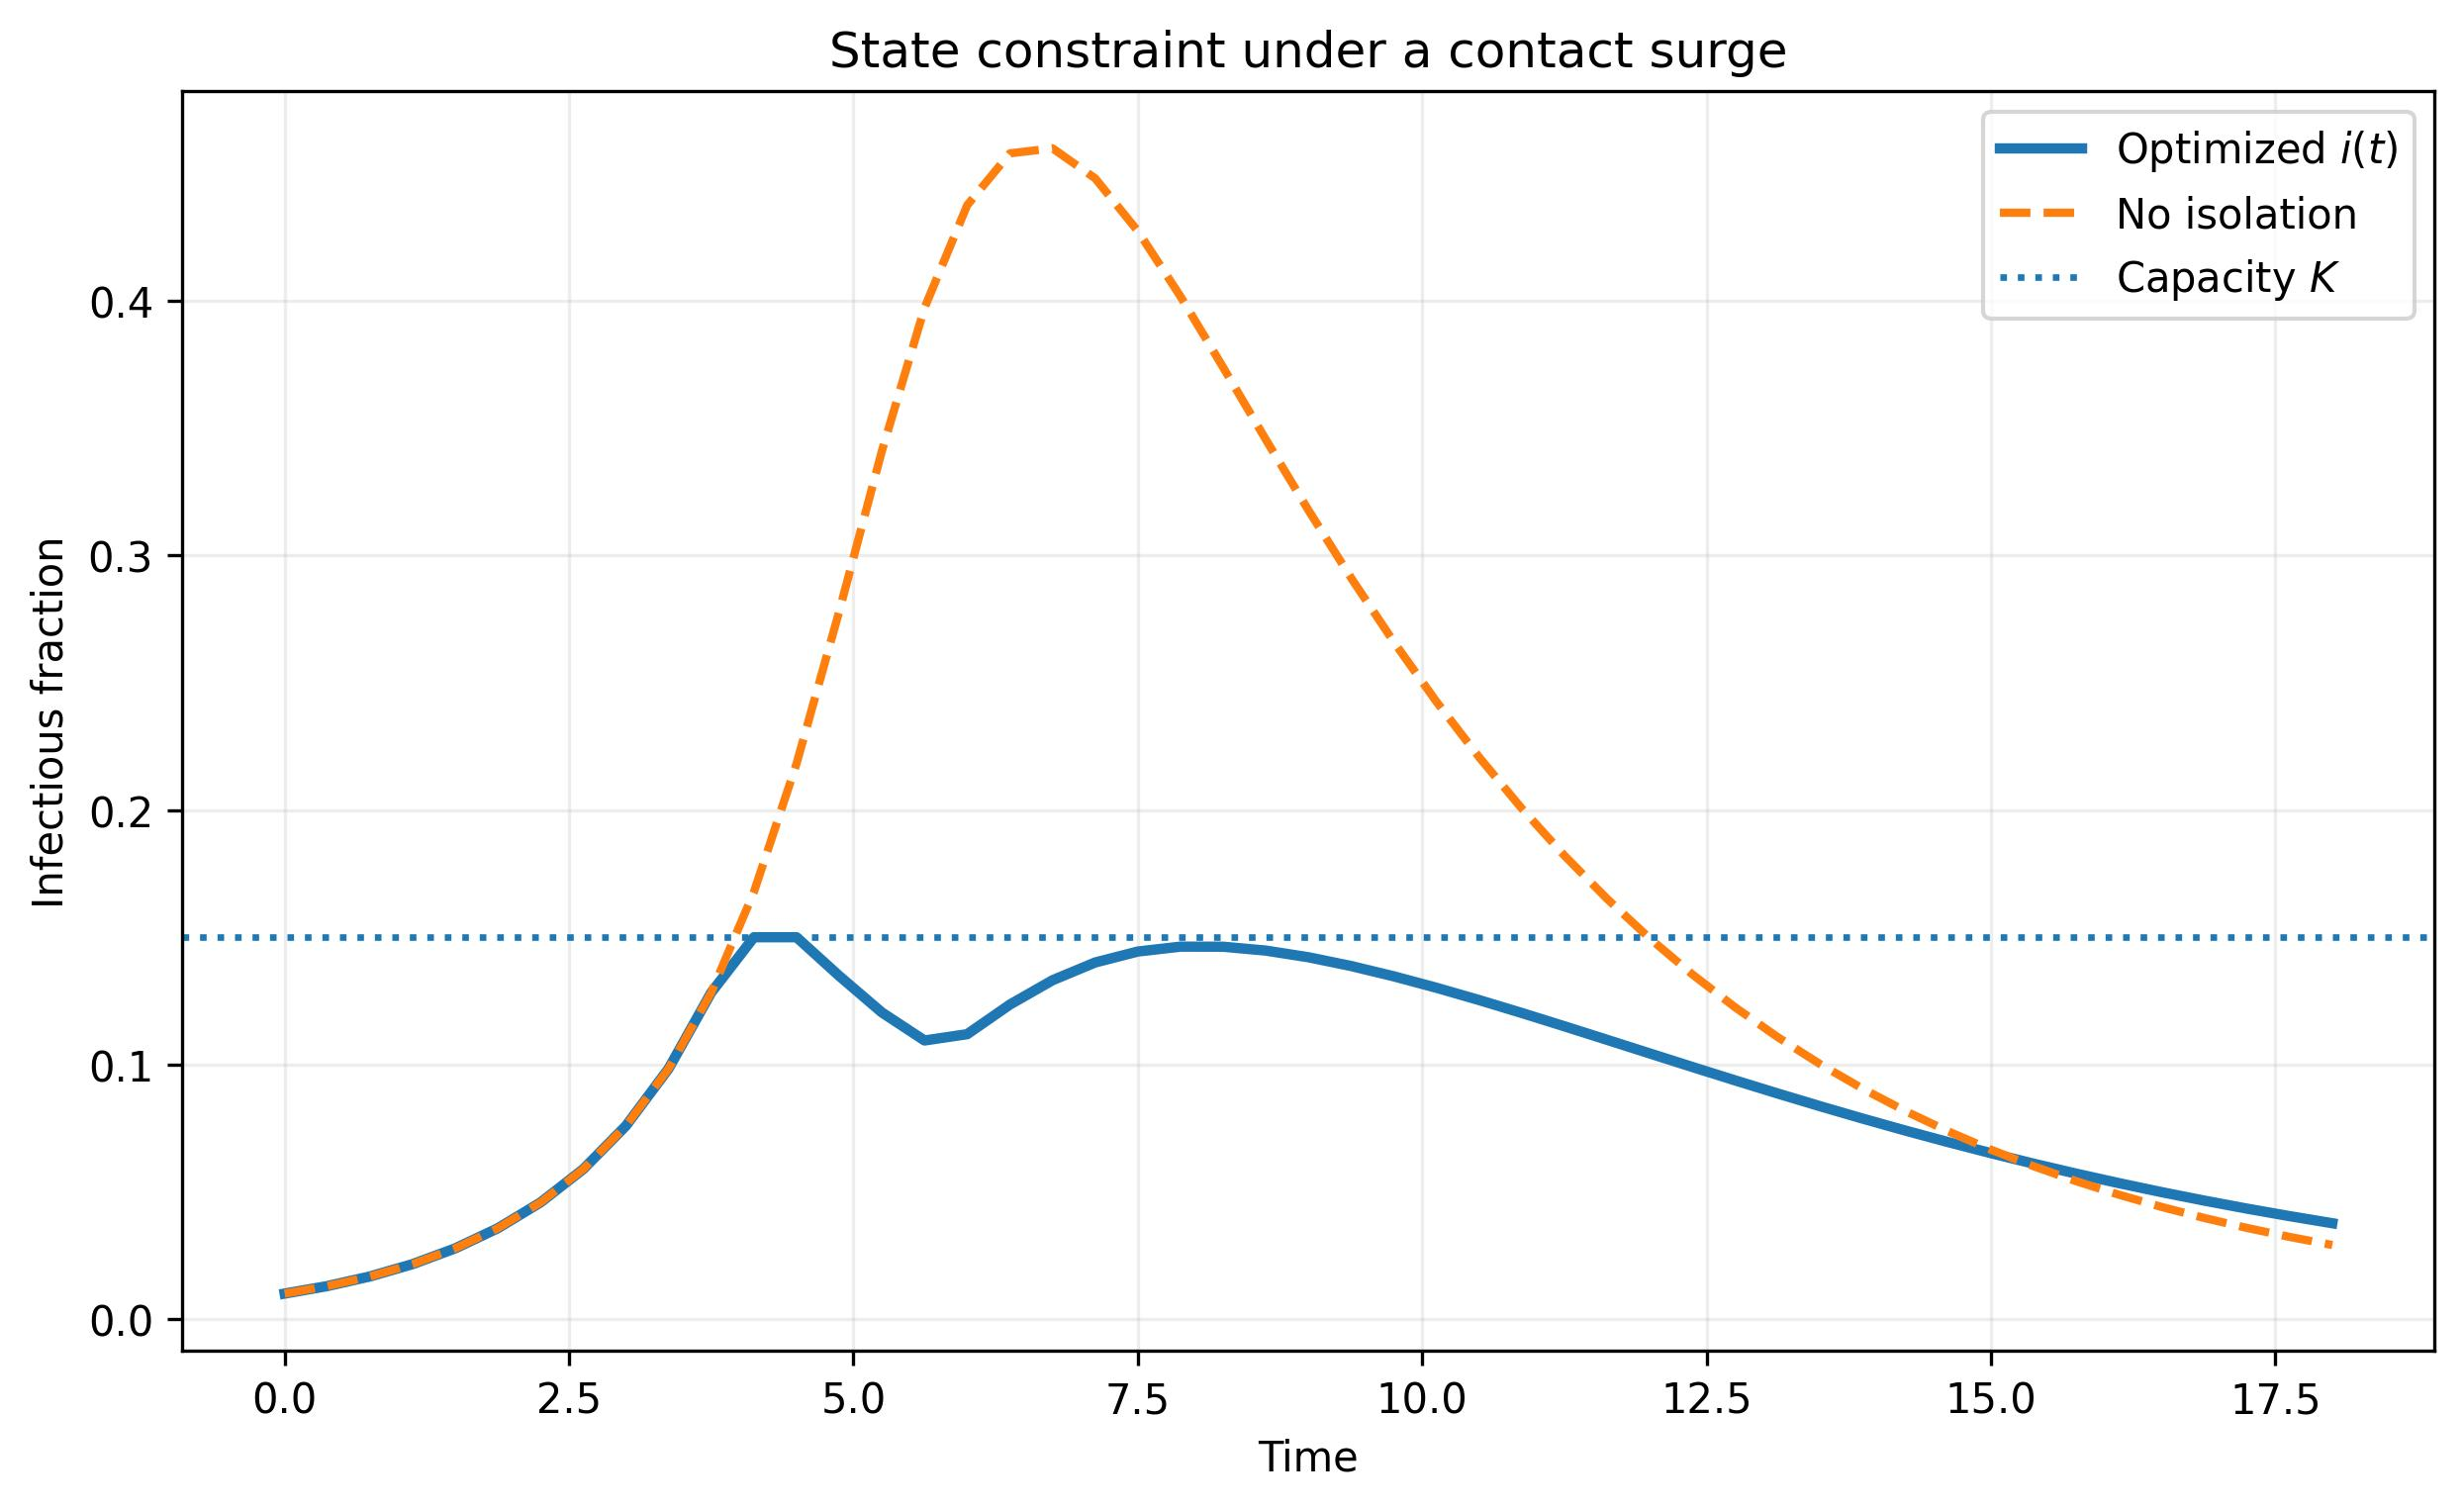
\includegraphics[width=0.92\textwidth]{Figure_10_time_varying_states.jpg}
\caption{原工程时变计算中的感染轨道。网格容量误差属于离散检查，不替代连续时间可行性和终端安全延拓的独立验证。}
\label{fig:time-states}\end{figure}
原工程报告 $\varepsilon=0.04$ 时目标值约为 $2.4280$、网格最大感染比例约为 $0.15$。
本次理论修订未重新求解该时变非线性规划，故将这些数值作为继承的离散计算结果，
不据此断言无穷时域最优性、连续轨道唯一性或正则化极限。
\FloatBarrier

\section{模型内的机制解释与理论边界}
\label{sec:limitations}
完全跟踪同时使感染生成归零、使未隔离易感者继续移出。
因此从内生阈值开始短时完全跟踪，比始终维持容量直至 $s=h$ 更节省本稿定义的成本。
这只是既定动力学与成本下的数学结论，不自动适用于含其他健康损失或资源约束的实际决策。
医疗容量 $K$、自然感染增长阈值 $h$、以及出现在不变量中的 $r$ 是不同的量；切换点由特征线上的 $\Theta$ 匹配确定。

\begin{remark}[本稿未完成、且未用于主定理的扩展证明]
\label{rem:unproved-extensions}
任意时变 $c(t)$ 的全域值函数构造、无穷时域终端处理和无条件唯一性未在本稿证明。
离散网格加密和 $\varepsilon\downarrow0$ 的收敛、时变高峰后的真实安全延拓也未证明。
$q_{\max}<1$、完全跟踪后残余感染生成、隔离者回流、联合控制以及参数不确定的情形需重新建立可行域和验证函数。
特别地，$q_{\max}<1$ 时，容量边界还必须满足 $q_{\max}\ge1-h/s$；
不能只把本稿的 $1$ 替换成 $q_{\max}$ 后沿用最优结构定理。
\end{remark}
\fi

\section{主要结论}
\label{sec:conclusions}
两个传播系数由同一跟踪比例耦合，但易感者移出与感染者生成对控制的响应方向不同。
在常接触率、线性成本、完整控制区间及正感染初值下，
本稿从有限可达域、非平凡切换曲线的完整参数化和全域分区出发，构造可行候选成本 $U$。
两种等待分支的统一梯度、内部匹配和容量水平集论证，给出对所有可测可行控制成立的验证不等式。
有限成本轨道的有限时间入安全集引理消除了额外终端假设，从而定理\ref{thm:verification}证明 $U=V$。

最优性与唯一性分别证明。平台上 Hamiltonian 的打平是结构性事实，
定理\ref{thm:unique-q}通过禁止提前离边、切换界面严格横穿及各段状态方程唯一性，
证明最优控制在全时间轴上几乎处处唯一。
允许零长度阶段后，非平凡结构为 $0\to1\to0$ 或 $0\to q_B\to1\to0$；
安全初值唯一采用 $q=0$。
基准初值的数值评价为 $J^*\approx1.52951116$，相对纯容量填充节省约 $3.10\%$。
数值计算只评价或核对解析构造，不承担全局充分性证明。

\ifdefined\TheoryOnly\else
时变接触率仅保留条件性的验证与唯一性讨论。
严格凸正则化给出的是固定状态和梯度下的唯一点态极小元，不能单凭此推出整个非线性控制问题全局唯一。
本稿未完成的扩展证明已在注\ref{rem:unproved-extensions}中列明，不作为常接触率主定理的结论。
\fi

\appendix
\section{完全跟踪成本导数的逐步计算}
\label{app:W-derivatives}
由
\[
G_0(s,i,\bar s)=i-\ell\ln s-a(\bar s)+\ell\ln\bar s=0
\]
及 $a'(\bar s)=(h-\bar s)/\bar s$，有
\[
\partial_{\bar s}G_0=-a'(\bar s)+\frac\ell{\bar s}
=\frac{\bar s-r}{\bar s}.
\]
于是
\[
-\frac\ell s+(\partial_{\bar s}G_0)\bar s_s=0,\qquad
1+(\partial_{\bar s}G_0)\bar s_i=0,
\]
从而得到 \eqref{eq:endpoint-derivatives}。
又 $\bar i_s=a'(\bar s)\bar s_s$、$\bar i_i=a'(\bar s)\bar s_i$。
对 $W=(\ln i-\ln\bar i)/h$ 求导即得
\[
W_s=-\frac1h\frac{a'(\bar s)\bar s_s}{\bar i}
=\frac{\ell(\bar s-h)}{hs(\bar s-r)\bar i},
\]
\[
W_i=\frac1h\left[\frac1i-\frac{a'(\bar s)\bar s_i}{\bar i}\right]
=\frac1h\left[\frac1i-\frac{\bar s-h}{(\bar s-r)\bar i}\right].
\]
这些导数首先属于指定策略成本 $W$，只有在完全跟踪分区完成验证后才同时是值函数的相应导数。

\section{容量边界成本积分的逐步计算}
\label{app:capacity-integral}
由 $\dot s=-cK(s-r)$，$\dd t=-\dd s/[cK(s-r)]$，得到
\[
C_B=\frac pK\int_{s_{\rm lo}}^{s_{\rm hi}}\frac{s-h}{s(s-r)}\dd s.
\]
作部分分式 $(s-h)/[s(s-r)]=A/s+B/(s-r)$。
比较系数得 $A+B=1$、$Ar=h$，所以
\[
A=\frac1{1-p},\qquad B=-\frac p{1-p}.
\]
代回并积分即得 \eqref{eq:boundary-cost}。

\section{证明依赖与校验口径}
\label{app:proof-scope}
常接触率证明的依赖顺序为：
状态正性和耗散；安全集及有限成本比较策略；有限成本入安全集；
完全跟踪可达域和成本；切换曲线几何；全域候选及达到性；梯度与拼接正则性；
沿任意轨道的验证；全局最优性；最后另证唯一性。
推论\ref{cor:one-dimensional-min}在全局验证之后陈述，不用候选策略族内的极小性替代全控制类比较。

相对于旧版本的 G1--G4，端点存在性现在由命题\ref{prop:reachable}及引理\ref{lem:tracking-region}处理；
曲线正则性和横截性由命题\ref{prop:Gamma-geometry}、推论\ref{cor:Gamma-labels}处理；
不滑行由引理\ref{lem:strict-crossing}处理。
局部 Lipschitz 性和终端处理分别由命题\ref{prop:regularity}及引理\ref{lem:finite-entry}证明。
任何一个数值扫描都不被用于证明这些全称命题。

本稿区分解析证明、符号恒等式检查、有限样本数值检查及排版编译检查。
后面三类检查可发现错误，但均不等价于对所有可行控制的解析证明，也不是形式化证明系统的验证。
本次修改范围、输入版本、实际执行的检查和未执行的检查见随附的修订记录。

\ifdefined\TheoryOnly\else
\section{原工程数值复现与本次修订的关系}
原工程公共解析模块仍为 \path{python/common_tracing.py}，总生成器为 \path{python/generate_data.py}。
原有命令为
\begin{lstlisting}
python python/generate_data.py
python python/generate_data.py --recompute-tv
python python/Figure_1_phase_geometry.py
python python/Figure_10_time_varying_states.py
\end{lstlisting}
本次修订不覆盖原图形、CSV 或这些求解程序；它们的旧日志不是本次新执行的验证结果。
随附 \path{verification/verify_revision.py} 独立核对本稿公式、分区及基准结果，
并输出机器可读报告。其取样检查不替代本稿的解析证明。
\fi
\bibliographystyle{plainnat}
\bibliography{references}
\end{document}
